\documentclass[a4paper, 11pt]{book}
% Font size (can be 10pt, 11pt or 12pt) and paper size (remove a4paper for US letter paper)

\usepackage[protrusion=true,expansion=true]{microtype} % Better typography
\usepackage{graphicx} % Required for including pictures
\usepackage{wrapfig} % Allows in-line images
\usepackage{mathpazo} % Use the Palatino font
\usepackage[T1]{fontenc} % Required for accented characters
\usepackage{amscd,amsmath}
\usepackage{tikz,stmaryrd}
\usepackage{latexsym,amsbsy,bbold, fullpage}
\usepackage{amssymb,amsthm,amsfonts}
\usepackage{pdfsync,yfonts}
\usepackage{tkz-graph}
\usepackage[all,pdf]{xy}
\usepackage{ctex}  %支持中文
\usepackage{titlesec}
\usepackage{color}
\usepackage{framed}
\usepackage{tcolorbox}
\usepackage{hyperref}
\usepackage{titlesec}



%%%%%%%%%%%%%%%%%%%%%%%%%交换图示例%%%%%%%%%%%%%%%%%%%%%%%%%%%%%%%%%%%%%%%%%%

%$$\xymatrix{
%\widetilde{K}(S(X\times Y))\ar[r]^{Si^*}
%&\widetilde{K}(S(X\vee Y))\ar[r]^{\delta}\ar[d]^{\cong}_{S\alpha}
%&\widetilde{K}(X\wedge Y)\ar[r]^{p^*}
%&\widetilde{K}(X\times Y)\ar[r]^{i^*}
%&\widetilde{K}(X\vee Y)\ar[d]^{\cong}_{\alpha}\\
%&\widetilde{K}(SX)\oplus \widetilde{K}(SY)\ar @{.>}[ul]^{S\eta}&&
%&\widetilde{K}(X)\oplus \widetilde{K}(Y)\ar @{.>}[ul]^{\eta}
%}$$

%%%%%%%%%%%_________The following are examples of pictures__________%%%%%%%%%

%\begin{figure}[ht]
%\centering
%\includegraphics[width=0.2\textwidth]{kdd.png}
%\caption{kuntion}
%\end{figure}

%%%%%%%%%%%%%%%%%%插入表格示意%%%%%%%%%%%%%%%%%%%%%%%%%%%%%%%%%%%%%%%%%%%%%%%%
%$$\begin{tabular}{|c|c|c|}   % |:竖线, l、c、r := 居左,居中,居右
%\hline
%直角边$a$ & 直角边$b$ & 斜边 $c$\\
%\hline
%3 & 4 & 5 \\
%\hline
%5 & 12 & 13 \\
%\hline
%7&24&25$\frac{1}{2\pi\sin\theta}$\\
%\hline
%\end{tabular}$$
%%%%%%%%%%%%%%%%%%%%%%%%%%%%%%%%%%%%%%%%%%%%%%%%%%%%%%%%%%%%%%%%%%%%%%%%%%%%%%%

\newcommand*{\vs}{\vspace{5pt}}
\newcommand*{\vsp}{\vspace{10pt}}
\newcommand*{\vspp}{\vspace{15pt}}
\newcommand*{\kong}{$\,\,\,\,\,\,\,$}
\newcommand*{\ad}{\text{ad}}

%\newcommand*{\ad}{\text{ad}}
\newcommand*{\Der}{\text{Der}}
\newcommand*{\ra}{\rightarrow}

\newcommand*{\defn}{\textit{Definition}:}
\newcommand*{\rmk}{\textit{Remark}:}
\newcommand*{\Example}{\textit{Example}}

\newcommand*{\R}{\mathbb{R}}
\newcommand*{\p}{\partial}
\newcommand*{\ten}{\otimes}

\newcommand*{\kai}{\CJKfamily{kai}}
\newcommand*{\hei}{\CJKfamily{hei}}
\newcommand*{\fs}{\CJKfamily{fs}}
\newcommand*{\song}{\CJKfamily{song}}

%%%%%%%%%%%%%%定理环境%%%%%%%%%%%%%%%%%%%%%%%

\newtheorem{thm}{定理}[section]
\newtheorem{lemma}{引理}[section]
\newtheorem{prop}{性质}[section]
\newtheorem{definition}{定义}[section]
\newtheorem{example}{例子}[section]
\newtheorem{rem}{注记}[section]
\newtheorem{cor}{推论}[section]
\newtheorem{claim}{断言}[section]
\newtheorem{intro}{导引}[section]
\newtheorem{prob}{习题}[section]


%%%%%%%%%%%%%%%%%%%%%%%%%%%%%%%%%%%%%%%%%%%%%%%%

\linespread{1.2} % Change line spacing here, Palatino benefits from a slight increase by default

\makeatletter
%\renewcommand\@biblabel[1]{\textbf{#1.}}
% Change the square brackets for each bibliography item from '[1]' to '1.'

\renewcommand{\@listI}{\itemsep=0pt}
% Reduce the space between items in the itemize and enumerate environments and the bibliography

\renewcommand{\maketitle}{
% Customize the title - do not edit title and author name here, see the TITLE block below
\begin{center} % Right align 可以换成 “flushleft”
{\Huge\@title} % Increase the font size of the title

\vspace{50pt} % Some vertical space between the title and author name

{\Large\@author} % Author name
\\\@date % Date

\vspace{20pt} % Some vertical space between the author block and abstract
\end{center}
}


\definecolor{shadecolor}{RGB}{237,255,224}


%\renewcommand{\abstractname}{摘要}
% Uncomment to change the name of the abstract to something else

\renewcommand{\bibname}{参考文献}
\renewcommand{\contentsname}{目录}
\renewcommand{\proofname}{证明}

\titleformat{\chapter}
  {\color{blue}
    \huge\bfseries}
  {第\,\thechapter\,章}
{1em}{}

\newcommand{\mchapter}[1]{
  \begin{shaded}
    \chapter{#1}
  \end{shaded}
}




\title{\textbf{曲豆豆的高等数学入门教程}\\$\,$\\% Title
卷一:基础架构} % Subtitle

\author{\textsc{曲豆豆\,\,\,主编} % Author
\\{\textit{豆瓣研究生小组\,\,\,\,\,荣誉出品}}} % Institution

\date{\today\\
第03-0.3稿}

%----------------------------------------------------------------------------------------
\begin{document}

\maketitle

%\begin{abstract}
%本讲义作为面向非数学专业者的入门,
%介绍近代数学的四大基本结构:
%序结构、代数结构、拓扑结构、测度结构,
%以及近代数学的表达、思考方式。
%\end{abstract}
\vspp

\begin{figure}[ht]
\centering
\includegraphics[width=0.7\textwidth]
  {figure/smg.jpg}

图:泛着神秘绿光的中国科学技术大学西校区

拍摄于2017.4.13 - 23:15
\end{figure}

\vspp

\rule[0pt]{14.3cm}{0.01em}\vs

\begin{centering}
本讲义由\LaTeX\ 排版,于GitHub开源\vsp

最新版本的讲义在
\href{https://github.com/qhn1121/Qu-Doudou-Project}
{这里}下载\vspp


欢迎经常访问
\href{https://github.com/qhn1121/Qu-Doudou-Project/commits}
{这里}以查看更新的细节

\end{centering}

\chapter*{前言}
\addcontentsline{toc}{chapter}{前言}

近代数学的一个特点是公理化、结构化。
代表近代数学的布尔巴基(Bourbaki)学派认为“数学是研究抽象结构的学科”,
这与恩格斯的观点“数学是关于现实世界数量关系和空间形式的科学”略有出入。
本讲义力图介绍近代数学中的四大基本结构:序结构、代数结构、拓扑结构、测度结构,
从而勾勒出近代数学基本框架,满足那些“想要多学一些数学”的爱好者们的基本需求,
并为其进一步学习近代数学奠定基础。

虽说声称是“零基础入门高等数学”,
本讲义其实并不是真正的“白手起家”,
还是要假定读者对一些基本的数学对象有直观的了解,
包括:实数的加减乘除运算、实数大小的比较,仅此而已。

事实上,近代数学基础完整的构建顺序大概是:命题逻辑$\rightarrow$
一阶谓词逻辑$\rightarrow$公理集合论$\rightarrow$自然数公理系统
$\rightarrow$实数理论。什么是自然数中的“0”,什么是“1”,
“自然数”是在集合论的框架下定义出来的,并不是“本来就有的”;
而自然数的加法运算也是定义出来的,
不再是初等数学那样子来源于日常生活经验,理所当然的。
这也是为什么罗素用了300多页才得到了自然数“1”的定义,这才是真正的“白手起家”。
有了自然数,之后再定义整数,
通过对整数环分式化来构造有理数,
再对有理数完备化来构造实数。

而本讲义跳过这个漫长的构建过程(但会在正文各处穿插地简要提一下),
直接假定读者知道什么是实数,以及实数的加减乘除、大小比较。
这样做的原因有两点,其一是避免讲义篇幅过长,
过分纠结于数学基础是枯燥乏味的,毕竟这个讲义不是专门的“数学基础”教材。
其二是为我们要介绍的抽象结构提供具体例子,比如讲到“偏序集”这个结构时,
实数配以通常的比较大小就是一个例子;
讲到“群”结构时,实数配以加法运算就是一个最基本的例子。
离开具体例子空谈抽象概念并不利于对数学概念的理解(当然格罗滕迪克Grothendieck是例外)。

由于这个讲义是笔者写着玩的,
且笔者水平有限,胡说八道之处在所难免。
希望读者批判性地看待本讲义中的某些论断。
另外由于匆忙成稿,笔误、语法错误应该也挺多的,
恳请批评指正。

最后,关于自然数的公理化构造,笔者恶搞《圣经:创世纪》中的一段,仅供娱乐,见下页。
\newpage

\textbf{致谢}

感谢笔者母校中国科学技术大学数学系的培养

感谢豆瓣小组提供平台

感谢一起编纂此讲义的小伙伴们

\vspp
\textbf{贡献者(豆瓣昵称,按拼音字母顺序排序)}

曲豆豆,王有为,在云上,子坚

\begin{centering}
\newcounter{density}
\setcounter{density}{0}
\begin{tikzpicture}
    \def\couleur{green}
    \path[coordinate] (0,0)  coordinate(A)
                ++( 144:6cm) coordinate(B)
                ++(72:6cm) coordinate(C)
                ++(0:6cm) coordinate(D)
                ++(-72:6cm) coordinate(E)
                                ;
    \draw[fill=\couleur!\thedensity] (A) -- (B) -- (C) --(D) -- (E) --  cycle;
    \foreach \x in {1,...,120}{%
        \pgfmathsetcounter{density}{\thedensity+5}
        \setcounter{density}{\thedensity}
        \path[coordinate] coordinate(X) at (A){};
        \path[coordinate] (A) -- (B) coordinate[pos=.05](A)
                            -- (C) coordinate[pos=.05](B)
                            -- (D) coordinate[pos=.05](C)
                            -- (E) coordinate[pos=.05](D)
                             -- (X) coordinate[pos=.05](E);
        \draw[fill=\couleur!\thedensity] (A)--(B)--(C)-- (D) --(E)  -- cycle;
    }
\end{tikzpicture}

\end{centering}
\begin{centering}

\tikzstyle{level 1}=[sibling angle=120]
\tikzstyle{level 2}=[sibling angle=60]
\tikzstyle{level 3}=[sibling angle=30]
\tikzstyle{every node}=[fill]
\tikzstyle{edge from parent}=[snake=expanding waves,segment length=1mm,
                              segment angle=10,draw]
\begin{tikzpicture}[grow cyclic,shape=circle,very thick,level distance=13mm,
                    cap=round]
\node {} child [color=\A] foreach \A in {red,green,blue}
    { node {} child [color=\A!50!\B] foreach \B in {red,green,blue}
        { node {} child [color=\A!50!\B!50!\C] foreach \C in {black,gray,white}
            { node {} }
        }
    };
\end{tikzpicture}
\end{centering}

\newpage

\begin{centering}
\begin{Large}
\textbf{《圣经:创世纪》节选}
\end{Large}\vsp
\large

起初,神创造逻辑。

逻辑是空虚的。

神的零运行在水面上,

这是平凡的。

神说,要有集合。

于是就有了集合。

神看集合是好的,

就将其公理化。

有集合,有运算,

就是一个代数结构。\vsp

神照自己的样子造人,

于是就有了0.

神在东方的伊甸建立了一个园子,

称之为群。

神将0安置在那里,

让它作幺元。

起初,伊甸园是平凡的。

神说,园中所有果子你可以随便吃。

只有后继树上果子,你不能吃。

因为你吃的时候必死。\vsp

神说,那人独居不好。

于是要为它造一个配偶。

神让0沉睡,取它的后继数1.

神把1带到伊甸园,

让它和0配对,

二人从此一起生活。

神教给它们加法的运算,

让它们可以互相交合。

0依然是伊甸园的单位元。

0的逆元是0,1的逆元是1,

0和1彼此交合则又得到1.\vsp

神所造的,

惟有皮亚诺比一切的活物更狡猾。

皮亚诺对1说,

神岂是真说不许你们吃园中所有树上的果子么?

1对皮亚诺说,

园中树上的果子我们可以吃,

唯有后继树上的果子不可,

免得我们死。

皮亚诺说,你们不会死。

神是怕你们吃了后继树上的果子,

能自己创造新的数。\vsp

皮亚诺告诉1它自己是怎么来的,

1对单调的只有0和1的加法已经厌烦。

它看后继树上的果子可做食物,

而且悦人眼目,是可喜爱的,

就摘下果子来吃了。\vsp

于是1对自己取了后继数,是为2.

1又摘下果子给2,2也吃了。

于是2对自己取了后继数,是为3.

很快,后继树下生成了所有正整数。。。

\end{centering}
\vspp

\begin{center}
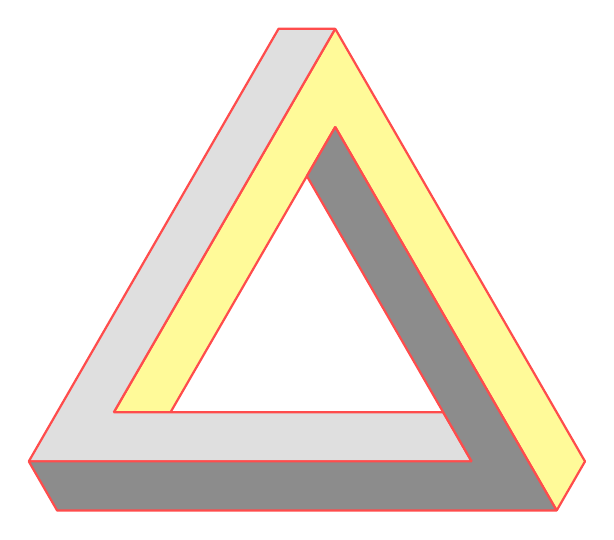
\begin{tikzpicture}[scale=0.8, line join=bevel]
    \pgfmathsetmacro{\a}{2.5}
    \pgfmathsetmacro{\b}{0.9}

    \tikzset{%
      apply style/.code     = {\tikzset{#1}},
      triangle_edges/.style = {thick,draw=red!70}
    }
    \foreach \theta/\facestyle in {%
        0/{triangle_edges, fill = yellow!40},
      120/{triangle_edges, fill = gray!25},
      240/{triangle_edges, fill = gray!90}%
    }{
      \begin{scope}[rotate=\theta]
        \draw[apply style/.expand once=\facestyle]
          ({-sqrt(3)/2*\a},{-0.5*\a})                     --
          ++(-\b,0)                                       --
            ({0.5*\b},{\a+3*sqrt(3)/2*\b})                -- % higher point	
            ({sqrt(3)/2*\a+2.5*\b},{-.5*\a-sqrt(3)/2*\b}) -- % rightmost point
          ++({-.5*\b},-{sqrt(3)/2*\b})                    -- % lower point
            ({0.5*\b},{\a+sqrt(3)/2*\b})                  --
          cycle;
        \end{scope}
      }	
\end{tikzpicture}
\end{center}








\tableofcontents

\mchapter{简明数理逻辑}

\begin{wrapfigure}{r}{0.4\textwidth}
\centering
\includegraphics[width=0.3\textwidth]{figure/psu}
\end{wrapfigure}数理逻辑是研究推理规则的数学分支。
而本章仅仅介绍数理逻辑的一些主要概念、
基本原理,不打算进一步深究。
在本章,我们常用的自然语言(中文 or English)
中的表达逻辑关系、推理证明的各个要素
将会被逐步地符号化,
即通过构造各种符号语言来代替自然语言,
最终得到完全由符号构成的形式语言。

为达到这个邪恶目的,
在本章第1-3节我们首先将关联词语
(两个命题之间的逻辑连接词)符号化,比如:
不但而且、虽然但是、因为所以、如果那么、只要就、只有才……等等;
而在第4-6节,我们将分析一个命题的内部构造,
将主体词、谓词、量词等“句子成分”也符号化。
最后在第7节,我们介绍在证明与整数有关的命题时常用的数学归纳法。


\section{命题与连接词}

\textbf{命题}是数理逻辑中的一个基本概念。
能够判断真假,非真即假的陈述句称为命题。

\begin{example}下列语句之中,
(1)-(3)都是命题,而(4)-(6)不是命题:

(1)加拿大位于北美洲;

(2)$1+1=3$;

(3)公元2333年元旦的北京是晴天;

(4)你脑子进屎了吗?

(5)让我们荡起双桨;

(6)这句话是假话。\label{examples of propositions}
\end{example}
\begin{proof}[Solution]
(1)(2)(3)都是可以判断真假的陈述句,
从而是命题,虽然(2)陈述的事实是荒谬的。
而对于(3),我们目前没有能力判断它到底是真还是假,
但它的真假性是客观存在的,这样的语句也是命题。

(4)(5)都不是陈述句,从而不是命题。
而(6)虽然是陈述句,但它的真假不确定,
假设它为真则推出它为假,由它为假又能推出它为真。
这种既不能为真也不能为假的陈述句,称为\textbf{悖论}。悖论不是命题。
\end{proof}

关于命题(3),与它类似的我们目前还没有能力判断真假的命题
有很多,比如著名的\textbf{哥德巴赫猜想}
“任何大于$4$的偶数都可以表示为两个素数的和”,
以及众多我们暂时没解决的数学猜想。\vsp

我们用小写拉丁字母,如$a,b,c,p,q,r$等,来表示命题。
如果一个命题为真,则称它为\textbf{真命题},
也称它的\textbf{真值}为1;若它为假,
则称此命题为\textbf{假命题},也称它的真值为0.\vsp

对于已经给定的一些命题,我们可以对这些命题进行一些操作,
来构造新的命题。接下来介绍常见的几种命题连接词。


\begin{definition}[否定连接词]
对于命题$p$,称命题$\neg p$为$p$的\textbf{否定式},
符号“$\neg$”称为否定连接词,读作“\textbf{非}”。
规定当$p$为真时,$\neg p$为假;$p$为假时$\neg p$为真。
\end{definition}

在自然语言中,命题“$\neg p$”可以表达为“$p$不成立”。
例如命题$p$表示“加拿大位于北美洲”,
则$\neg p$表示“加拿大不位于北美洲”。

\begin{definition}[合取连接词]
对于两个命题$p,q$,称命题
“$p\wedge q$”为$p$与$q$的\textbf{合取式},
符号“$\wedge$”称为合取连接词,读作“\textbf{且}”。
规定当$p,q$全都是为真命题时,$p\wedge q$为真命题;
当$p,q$之中至少有一个是假命题时,$p\wedge q$为假命题。
\end{definition}
对于两个命题$p,q$,$p\wedge q$用自然语言可以描述为
“$p$与$q$同时成立”、“$p$与$q$全都正确”、“$p$并且$q$”、
“虽然$p$但是$q$”、“不仅$p$而且$q$”、
“both $p$ and $q$ are true”等等。

特别注意自然语言中的“但是”和“并且”,
其实表达的都是$\wedge$的意思,指两者同时成立。

\begin{definition}[析取连接词]
对于两个命题$p,q$,
称命题“$p\vee q$”为$p$与$q$的\textbf{析取式},
符号“$\vee$”称为析取连接词,读作“\textbf{或}”。
规定当$p,q$全都是为假命题时,$p\vee q$为假命题;
当$p,q$之中至少有一个是真命题时,$p\vee q$为真命题。
\end{definition}
对于两个命题$p,q$,
“$p\vee q$”在自然语言中常称为“$p$或者$q$”.
然而特别注意,“或者”这个词在汉语中有歧义,
在有些语境下表示“两者当中有且只有一个成立”,
例如“你滚蛋,或者我滚蛋”。但是在数理逻辑中,
“或者”指的是两者至少有一个成立就可以(两者都成立那更好)。

\begin{definition}[蕴含连接词]
对于两个命题$p,q$,称命题“$p\rightarrow q$”为$p$与$q$的\textbf{蕴含式},
符号“$\rightarrow$”称为蕴含连接词,读作“\textbf{蕴含}”。
规定当$p$为真命题并且$q$为假命题时,$p\rightarrow q$为假命题;
而其余3种情况时$p\rightarrow q$为真命题。
\end{definition}

对于两个命题$p,q$,“$p\rightarrow q$”
在自然语言和今后我们要学习的数学当中,有
“如果$p$那么$q$”,“$p$仅当$q$”,“$p$推出$q$”,
“因为$p$所以$q$”,“只要$p$就有$q$”,
“只有$q$才会有$p$”,“除非$q$否则$p$”、
“$p$是$q$的\textbf{充分条件}”,
“$q$是$p$的\textbf{必要条件}”等
看似迥异的表述方式。

上述诸多表达方式在数理逻辑中其实表达的都是“蕴含”的含义,
这需要慢慢体会。

蕴含连接词也许是在本节所讲的所有连接词中最令初学者费解的一个。
为帮助读者理解,我们举一些例子来说明:

\begin{example}研究下列命题。
虽然它们表达的含义荒诞至极,
但在数理逻辑的意义下它们都是真命题:

(1)因为所有人都吃过屎,所以地球围绕太阳公转。

(2)如果1+1=3,那么猪会飞。

(3)只有沙漠能下暴雨,大海才会亲吻鲨鱼。

(4)只要2是奇数,公元2333年元旦的北京就是晴天。
\end{example}
\begin{proof}
我们依次来分析这些命题:

(1)我们用字母$p$来表示“所有人都吃过屎”,用$q$来表示“地球围绕太阳公转”。
则命题(1)用符号表达为“$p\rightarrow q$”.由于$p$是假命题,$q$是真命题,
所以根据蕴含连接词"$\rightarrow$"的定义可知$p\rightarrow q$为真命题。

(2)该命题为“$(1+1=3)\rightarrow\text{猪会飞}$”。
由于“1+1=3”是假命题,“猪会飞”也是假命题,从而命题(2)是真命题。

(3)该命题为“大海亲吻鲨鱼$\rightarrow$沙漠下暴雨”,
蕴含连接词的前后两端都是假命题,从而这个命题是真命题。

(4)该命题为“2是奇数$\rightarrow$公元2333年元旦的北京是晴天”。
我们知道“2是奇数”是假命题。虽然我们并没有能力判断公元2333年那件事的真假,
但是从蕴含连接词的定义可以看出,
对于一个由蕴含连接词连接的复合命题$p\rightarrow q$,只要$p$是假命题,
那么无论$q$是真是假,$p\rightarrow q$一定是真命题。从而命题(4)是真命题。
\end{proof}

要特别注意,在日常生活的自然语言中,
“如果$p$那么$q$”中的$p,q$之间通常有内在的联系,
因果联系、依赖关系等等。
而数理逻辑研究的是抽象的推理,
“命题”本身是一个剥离于现实世界的抽象的概念,
我们谈论命题“$p\rightarrow q$”时,
$p$与$q$之间可以毫无任何联系。
命题“$p\rightarrow q$”的真假性,只与$p,q$两者的真假性有关,
而与它们所表达的实际意义之间有何内在联系无关。
这对于其它几个逻辑连接词,也都是如此。

我们再看一些关于蕴含连接词的例子:

\begin{example}
甲、乙两个人比赛,甲对此信心满满,
说:“如果我输了,我给你100块钱。”
试将命题“如果甲输,那么甲给乙100块钱”符号化,
并讨论该命题何时为假命题。
\end{example}
\begin{proof}[Solution]
此命题为“甲输$\rightarrow$甲给乙100块钱”。
只有当甲输了但是甲没给乙100块钱时,
甲所讲的这个命题才是假的。
特别注意当甲赢了时候(即“甲输”为假命题),
无论甲有没有给钱,那句话都是真命题。
\end{proof}

这个实际例子也许能够帮助初学者理解
为什么要规定当前提$p$为假命题时
$p\rightarrow q$ 一定是真命题。事实上,
再以后的学习中,我们会接触到更多
抽象的结构(比如拓扑空间、概率空间等),
它们的严格定义会令初学者费解。之所以要如此定义,
是因为这样定义出来的东西具有我们所希望的性质
——这正是近代数学的特色之一。
我们在下一节会介绍“所希望的性质”具体是什么
(见下一节的定理\ref{prop-dengzhi-gongshi-3})。
\begin{example}假设你是人(这是确凿无疑的),
试判断下列命题的真假:

(1)如果你是人,那么你不是人。

(2)如果你不是人,那么你是人。

(3)你是人,并且你不是人。

(4)除非你是人,否则你不是人。
\end{example}

\begin{proof}[Solution]
我们用字母$p$表示命题“你是人”,
则$p$为真命题(希望读者承认这个事实)。
则上述4个命题用符号来表达,分别为
$$p\rightarrow (\neg p)\,\,\,,\,\,\,
(\neg p)\rightarrow p\,\,\,,\,\,\,
p\wedge(\neg p)\,\,\,,\,\,\,
(\neg p)\rightarrow p$$
由相应连接词的运算规则,
不难得出(1)(3)为假命题,(2)(4)为真命题。
\end{proof}

\begin{definition}[等价连接词]
对于两个命题$p,q$,称命题“$p\leftrightarrow q$”为$p$与$q$的\textbf{等价式},
符号“$\leftrightarrow$”称为等价连接词,读作“\textbf{等价于}”。
规定当$p,q$真值相同时$p\leftrightarrow q$为真命题;
真值相反时$p\leftrightarrow q$为假命题。
\end{definition}
在自然语言以及数学中,常用“$p$\textbf{当且仅当}$q$”、
“$p$是$q$的\textbf{充要条件}”、
“$p$ \textbf{if and only if} $q$”
来表达命题“$p\leftrightarrow q$”.\vsp

以上是常见的五种逻辑连接词。
我们将由连接词组成的复合命题的真假性
总结为如下\textbf{真值表}:

$$\begin{tabular}{|c||c|c|c|c|c|}
\hline
$p\,\,q$ & $\neg p$ & $p\wedge q$ & $p\vee q$
& $p\rightarrow q$ & $p\leftrightarrow q$\\
\hline
$0\,\,0$ & 1 & 0 &0&1&1 \\

$0\,\,1$ & 1 & 0 &1&1&0 \\

$1\,\,0$ & 0 & 0 &1&0&0 \\

$1\,\,1$ & 0 & 1 &1&1&1 \\
\hline
\end{tabular}$$

例如,从表中第一行可以看出,
当$p,q$都是假命题(真值为0)时,
$\neg p$、$p\wedge q$、$p\vee q$、
$p\rightarrow q$、$p\leftrightarrow q$的真值
分别为1、0、0、1、1.\vsp

由简单的命题,以及各种逻辑连接词,可以构造出复杂的命题。
例如对于命题$p,q,r,s$,我们可以去谈论诸如
$$((\neg p)\vee r)\wedge(s\leftrightarrow q)$$
这样的复杂命题。这种命题的真假性完全由
$p,q,r,s$之中每一个命题的真假性决定。\vs

我们再简单提一下逻辑连接词运算的\textbf{优先级}。
与实数加减乘除运算规则“先乘除后加减,
有括号先算括号里面的”类似,
我们也约定各种逻辑连接词的优先级。规定优先顺序为
$$\neg\,>\,\wedge\,>\,\vee\,>\,\rightarrow\,>\,\leftrightarrow$$

例如,命题$\neg p\vee q$确切地说应该是
$(\neg p)\vee q$,而不是$\neg(p\vee q)$.
再比如,命题$p\vee q\leftrightarrow r\wedge s$所表达的含义是
$(p\vee q)\leftrightarrow (r\wedge s)$,
而不是$((p\vee q)\leftrightarrow r)\wedge s$.

在以后,我们尽量避免依靠这个优先级约定规则,
而是尽可能多加括号减少歧义。\vsp

本节最后,简单提一下命题变量。
回顾在初等数学中我们用字母(比如$x$)表示实数。
在一些语境下,$x$是一个确定的数,
而在有些语境下字母$x$代表的数不确定——
这正是\textbf{常量}与\textbf{变量}的区别。
比如“$x^2+1$”,在某些语境下,$x$是一个确定的数,
那$x^2+1$就是一个确定的数;而在另一些语境下,
$x^2+1$是一个公式,我们给$x$赋以特定的值,
就会得到$x^2+1$的一个值。
特别注意一个字母到底代表常量还是变量,
需要依靠事先约定以及语境来判断。\vs

而命题逻辑与之完全类似。我们用字母来表示一个命题。
命题也有\textbf{命题常量}与\textbf{命题变量}之分。
前者为某个确定的命题,而后者是一个抽象的符号,
可以被赋以确定的命题。

\section{命题逻辑等值演算}
现在,我们已经用字母来表示命题
(包括命题常量与命题变量),
并且定义了几个常见的逻辑连接词。
本节开始,我们研究命题逻辑的运算。

\begin{definition}[命题公式]
由命题常量、命题变量、逻辑连接词、括号$()$按照某些逻辑关系
所排列而成的符号串称为命题公式。具体地,“某些逻辑关系”指的是:

(1)对于单个命题常量或者命题变量$p$,
由符号$p$自身构成的符号串是命题公式。

(2)如果符号串$A,B$都是命题公式,那么符号串
$$\neg A$$
$$A\vee B$$
$$A\wedge B$$
$$A\rightarrow B$$
$$A\leftrightarrow B$$
都是命题公式。

(3)对于符号串$A$是命题公式,那么符号串“$(A)$”也是命题公式。
\label{命题公式的概念}
\end{definition}

注意“命题公式”这个概念是\textbf{归纳定义}
(或者叫\textbf{递归定义})的。
通俗地说,命题公式是由有限多个命题常量、有限多个命题变量,
经过命题连接词的有限多步连接,所构成的符号串。

例如,我们用字母$p$来表示命题“地球绕太阳公转”,那么符号串
$$((\neg p)\vee q)\leftrightarrow(r\rightarrow p)$$
是一个命题公式。其中$q,r$是命题变量,而$p$是命题常量。
这个命题公式含有2个命题变量。特别注意,命题公式可以不含有命题变量。

再注意一点,命题连接词除了我们提到的5种
(否定、合取、析取、蕴含、等价)之外,
还有无数多种;只不过这5种比较“常用”,
自然语言中存在表达其含义的词汇。
而其它一些连接词,它表达的逻辑关系是“无法言说的”
(无法用正常的“人话”轻易讲清楚),
自然语言在其面前苍白无力。
我们在本章习题中会提到一些其它的连接词。
事实上,在习题中我们还将证明“$\neg,\vee$”
这两个连接词在某种意义下已经“足够用”了。

对于用这5种连接词之外的连接词来连接的字符串,
我们也认为是命题公式。这在本章习题中会略加讨论。

\begin{definition}[命题公式的赋值]
设字符串$A=A(p_1,...,p_n)$是含有$n$个命题变量$p_1,p_2,...,p_n$的
一个命题公式。对每个$p_1,...,p_n$各指定一个真值,
称为命题公式$A$的一个\textbf{赋值}(或者称为“\textbf{诠释}”)。
\end{definition}

容易知道,对于含有$n$个命题变量的命题公式$A$,
$A$总共有$2^n$种不同的赋值。(这是因为对于每个命题变量,
要么赋以它真值0,要么赋以它真值1,
一共2种选择;而共有$n$个变量,从而总共
$2\times 2\times...\times2=2^n$种赋值)

回顾上一节出现的\textbf{真值表}。对于命题公式,
我们可以穷尽它所有可能的赋值,
并把每一种赋值及其结果一一列出。

\begin{example}我们考虑关于命题变量$p,q,r$的下述三个命题公式
$$A:=p\rightarrow (q\rightarrow r)$$
$$B:=(p\wedge q)\rightarrow r$$
$$C:=(p\rightarrow q)\rightarrow r$$
试讨论它们所有可能的赋值,并总结为真值表。
\label{proposition formula}
\end{example}
\begin{proof}[Solution]
逐一讨论所有可能的$2^3=8$种赋值,总结为下表:

$$\begin{tabular}{|c||c|c|c|}   % |:竖线, l、c、r := 居左,居中,居右
\hline
$p\,\,q\,\,r$ & $p\rightarrow (q\rightarrow r)$
& $(p\wedge q)\rightarrow r$ & $(p\rightarrow q)\rightarrow r$ \\
\hline
$0\,\,0\,\,0$ & 1 & 1 & 0  \\
$0\,\,0\,\,1$ & 1 & 1 & 1  \\
$0\,\,1\,\,0$ & 1 & 1 & 0  \\
$0\,\,1\,\,1$ & 1 & 1 & 1  \\
$1\,\,0\,\,0$ & 1 & 1 & 1  \\
$1\,\,0\,\,1$ & 1 & 1 & 1  \\
$1\,\,1\,\,0$ & 0 & 0 & 0  \\
$1\,\,1\,\,1$ & 1 & 1 & 1  \\
\hline
\end{tabular}$$
按照相应逻辑连接词的运算规则,读者可自行验证上述结果。
\end{proof}

注意观察上述真值表的(从双竖线右边起)
第1、2列,发现它们完全相同。
也就是说,对于公式
$p\rightarrow (q\rightarrow r)$
与$(p\wedge q)\rightarrow r$,
无论对变量$p,q,r$赋予哪些真值,
所得到的命题的真值都相同。

与初等数学类比一下,这就好比含有变量$x,y$的两个表达式
$$2(x+2y)\,\,\,\,,\,\,\,\,2x+4y$$
无论对$x,y$赋予什么值,所得到的结果都相等。
(但实数有无限多个,我们无法一一列出上述式子所有可能的赋值,
总结成类似的真值表。
所以在这种意义下,命题逻辑比初等代数简单得多。)\vs

在初等数学中,我们并不是通过暴力验证对变量$x,y$的每一种可能的赋值,
来证明$2(x+2y)$与$2x+4y$是“相等”的
(事实上暴力穷举是不现实的,毕竟实数有无限多个),
而是通过一些\textbf{运算律};而命题逻辑的简单之处在于
我们可以暴力地验证所有可能的赋值来说明两个命题公式其实是“相等”的。
事实上暴力验证可以交给计算机来完成。

\begin{definition}[命题公式的分类]
对于含有$n$个$(n\geq0)$命题变量的命题公式$A=A(p_1,...,p_n)$,

(1)称$A$为\textbf{重言式}(或者\textbf{永真式}),
如果在$A$的任何赋值下,$A$的结果都为真;

(2)称$A$为\textbf{矛盾式}(或者\textbf{永假式}),
如果在$A$的任何赋值下,$A$的结果都为假;

(2)称$A$为\textbf{可满足式},
如果存在$A$的某个赋值,使得$A$的结果为真;
\end{definition}

从定义容易看出,重言式一定是可满足式。

顺便提一下$n=0$这种\textbf{平凡}(trivial)的情形,
即$A$为含有0个命题变量的命题公式的情形。
此时$A$无非就是一个命题常量。
$A$为重言式当且仅当$A$为真命题当且仅当$A$为可满足式;
$A$为矛盾式当且仅当$A$为假命题。\vs

判断一个命题公式是否为重言式、可满足式、矛盾式,
我们可以用真值表的方法。
即,穷尽所有可能的赋值。
例如,在刚才的例子\ref{proposition formula}
之中出现的三个命题公式都是可满足式,
都不是重言式——从它们的真值表中能轻易看出来。

\begin{definition}[命题公式的等值]
对于含有$n$个命题变量$p_1,...,p_n$的两个命题公式$A,B$,
称$A$与$B$\textbf{等值},如果在所有可能的$2^n$个赋值之下,它们的真值都相同。
此时记作$A\Leftrightarrow B$.
\end{definition}
例如,例子\ref{proposition formula}
之中的两个命题公式$A,B$是等值的,
这从真值表中可以看出来。
用符号语言表示为
$$[p\rightarrow (q\rightarrow r)]
\Leftrightarrow [(p\wedge q)\rightarrow r]$$
特别需要注意的是,符号“$\Leftrightarrow$”并不是逻辑连接词,
不要与$\leftrightarrow$混淆。不过它们两者之间有如下联系:

\begin{thm}对于含有$n$个命题变量
$p_1,...,p_n$的命题公式$A,B$,则
$A\Leftrightarrow B$当且仅当
$A\leftrightarrow B$是重言式。
\end{thm}
\begin{proof}
这根据“等值$\Leftrightarrow$”、“重言式”、
“命题连接词$\leftrightarrow$”的定义,
直接得到。几乎是显然的。
不过在此还是要详细写一下证明,给初学者。

一方面在$A\Leftrightarrow B$的条件下,
我们将证明$A\leftrightarrow B$是重言式。
根据重言式的定义,我们只需要证明,
对于变量$p_1,...,p_n$的任何赋值,得到的命题
$A(p_1,...,p_n)\leftrightarrow B(p_1,...,p_n)$是真命题。
而这是因为,由于$A\Leftrightarrow B$,从而
$A(p_1,...,p_n)$与$B(p_1,...,p_n)$的真值总是相同,
因此由逻辑连接词$\leftrightarrow$
的运算规则知$A(p_1,...,p_n)
\leftrightarrow B(p_1,...,p_n)$是真命题,
这对任何赋值都成立。从而$A\leftrightarrow B$是重言式。

另一方面,我们还要证明在$A\leftrightarrow B$是重言式的条件下,
有$A\Leftrightarrow B$.方法完全类似
(刚才的证明过程处处可逆),读者自行完成。
\end{proof}

\begin{rem}[关于命题公式的命题变量个数]
对于两个命题公式$P,Q$(一般地,可以是任意有限多个命题公式),
设它们总共具有$n$个命题变量$p_1,...,p_n$.

注意到,我们允许发生以下情况:
$A,B$之中的某一个命题公式(不妨为$A$)
\underline{不全含}这些命题变量。
例如,$A$只含有命题变量$p_1,...,p_s$,
其中$1\leq s<n$,而不含有$p_{s+1},...,p_{n}$.
此时,称命题变量$p_{s+1},...,p_{n}$为
命题公式$A$的\textbf{哑元}。
\end{rem}

事实上,对于含有$n$个命题变量
$p_1,...,p_n$的命题公式$P$,
则对于除了$p_1,...,p_n$之外的任何一个命题变量$q$,
$q$都可以被视为命题公式$P$的哑元。

\begin{example}[哑元的简单例子]
考虑两个命题公式
$$P:=p\rightarrow q$$
$$Q:=q\vee r$$
则$P$与$Q$总共含有$p,q,r$三个命题变量。
容易知道,命题变量$r$是命题公式$P$的哑元;
类似地,$p$是$Q$的哑元。
\end{example}

此时,我们也认为$P,Q$都是关于$p,q,r$
三个命题变量的命题公式
(虽然实际上它们都只含有2个命题变量,
不全含所有的命题变量)。

对含有哑元的命题公式的赋值,
赋值后的真值与哑元的取值无关。
具体在本例中,命题公式$P,Q$
(都视为含有3个命题变量的命题公式)的真值表如下:

$$\begin{tabular}{|c||c|c|}
\hline
$p\,\,q\,\,r$&$p\rightarrow q$&$q\vee r$\\
\hline
$0\,\,0\,\,0$&1&0\\
$0\,\,0\,\,1$&1&1\\
$0\,\,1\,\,0$&1&1\\
$0\,\,1\,\,1$&1&1\\
$1\,\,0\,\,0$&0&0\\
$1\,\,0\,\,1$&0&1\\
$1\,\,1\,\,0$&1&1\\
$1\,\,1\,\,1$&1&1\\
\hline
\end{tabular}$$

通过比较真值表可以看出,
命题公式$P$与$Q$不等值。

也就是说,即使两个命题公式$P,Q$所含有的命题变量不相同,
我们也可以去谈论它们是否等值——
只需要把它们都视为含有两者全部的命题变量的命题公式,
不妨含有哑元。

在以后,为方便起见,
我们默认命题公式中可以含有哑元。

\begin{rem}命题常量可以视为含有0个命题变量的命题公式。
我们令“1”为某个给定的真命题,
它也被视为一个取值恒为1的的命题公式,
也就是重言式;也习惯用“0”来表示某个给定的假命题,
它也被视为一个取值恒为0的命题公式,也就是矛盾式。
\end{rem}

这有一些记号混用,具体含义需要读者依靠语境判断。
对于一个含有命题变量$p_1,...,p_n$的命题公式$P$,
如果$P$是重言式,则我们记
$$P\Leftrightarrow 1$$

在上式中,“1”被视为含有$n$个命题变量
$p_1,...,p_n$的重言式。
$p_1,...,p_n$都是命题公式“1”的哑元。
类似地,“$P$是矛盾式”也记作“$P\Leftrightarrow0$”,
读者可以望文生义。\vsp

接下来将介绍一些常见的命题公式
(可以含有哑元)的等值式。

\begin{thm}[基本的命题公式等值式I]\label{prop-dingzhi-gongshi-1}
设$A$为任意的命题公式,则下列成立:

(1)零律:$$A\vee1\Leftrightarrow1$$
$$A\wedge0\Leftrightarrow0$$

(2)同一律:$$A\wedge1\Leftrightarrow A$$
$$A\vee0\Leftrightarrow A$$

(3)幂等律:$$A\Leftrightarrow A\vee A$$
$$A\Leftrightarrow A\wedge A$$

(4)双重否定律:$$A\Leftrightarrow \neg(\neg A)$$

(5)排中律:$$A\vee\neg A\Leftrightarrow1$$

(6)矛盾律:$$A\wedge\neg A\Leftrightarrow0$$

\end{thm}
\begin{proof}
这些都是显然的,直接用真值表验证即可
(考虑$A$的真值为$0,1$的两种情况即可)。

也请读者思考上述等值式中出现的“0”、"1"的具体含义。
它们都被视为含有哑元的命题公式。
\end{proof}

特别注意,上述等值式中的$A$可以被替换为任何命题公式。
比如令$A$为含有3个命题变量的命题公式
$(p\rightarrow q)\rightarrow r$,则
幂等律(3)变为
$$(p\rightarrow q)\rightarrow r
\Leftrightarrow [(p\rightarrow q)\rightarrow r]
\vee [(p\rightarrow q)\rightarrow r]$$
$$(p\rightarrow q)\rightarrow r
\Leftrightarrow [(p\rightarrow q)\rightarrow r]
\wedge [(p\rightarrow q)\rightarrow r]$$
这仍然是命题等值式。
上述$p,q,r$也可以继续被替换为更复杂的命题公式。

\begin{thm}[基本的命题公式等值式II]\label{prop-dengzhi-gongshi-2}
对于任何命题公式$A,B,C$,则下列等值式成立:

(7)交换律:$$A\wedge B\Leftrightarrow B\wedge A$$
$$A\vee B\Leftrightarrow B\vee A$$

(8)结合律:$$(A\wedge B)\wedge C\Leftrightarrow A\wedge (B\wedge C)$$
$$(A\vee B)\vee C\Leftrightarrow A\vee (B\vee C)$$

(9)分配律:
$$(A\wedge B)\vee C\Leftrightarrow (A\vee C)\wedge (B\vee C)$$
$$(A\vee B)\wedge C\Leftrightarrow (A\wedge C)\vee (B\wedge C)$$

(10)吸收律:
$$A\vee (A\wedge B)\Leftrightarrow A$$
$$A\wedge (A\vee B)\Leftrightarrow A$$

(11)德摩根律:
$$\neg(A\vee B)\Leftrightarrow\neg A\wedge\neg B$$
$$\neg(A\wedge B)\Leftrightarrow\neg A\vee\neg B$$

\end{thm}

\begin{proof}
对命题公式$A,B,C$被赋值之后所得到的命题的真假进行讨论,
用真值表暴力验证即可。

我们先来看交换律(7).列出真值表,见下表:
$$\begin{tabular}{|c||cc|cc|}   % |:竖线, l、c、r := 居左,居中,居右
\hline
$A\,\,B$ & $A\wedge B$ & $B\wedge A$ & $A\vee B$ & $B\vee A$\\
\hline
$0\,\,0$ & 0 & 0 & 0 & 0  \\
$0\,\,1$ & 0 & 0 & 1 & 1  \\
$1\,\,0$ & 0 & 0 & 1 & 1  \\
$1\,\,1$ & 1 & 1 & 1 & 1  \\
\hline
\end{tabular}$$
观察此真值表各列,容易发现相应的等值关系。

接下来看(8)结合律,我们暴力列出如下真值表:

$$\begin{tabular}{|c||cc|cc|}
\hline
$A\,\,B\,\,C$ & $(A\wedge B)\wedge C$ & $A\wedge (B\wedge C)$
& $(A\vee B)\vee C$ & $A\vee (B\vee C)$\\
\hline
$0\,\,0\,\,0$ & 0 & 0 & 0 & 0  \\
$0\,\,0\,\,1$ & 0 & 0 & 1 & 1  \\
$0\,\,1\,\,0$ & 0 & 0 & 1 & 1  \\
$0\,\,1\,\,1$ & 0 & 0 & 1 & 1  \\
$1\,\,0\,\,0$ & 0 & 0 & 1 & 1  \\
$1\,\,0\,\,1$ & 0 & 0 & 1 & 1  \\
$1\,\,1\,\,0$ & 0 & 0 & 1 & 1  \\
$1\,\,1\,\,1$ & 1 & 1 & 1 & 1  \\
\hline
\end{tabular}$$
分配律、吸收律、德摩根律的证明完全类似,留给读者完成。
\end{proof}

关于等价、蕴含连接词,还有如下等值式:

\begin{thm}[基本的命题公式等值式III]\label{prop-dengzhi-gongshi-3}
设$A,B$为任意的命题公式,则成立下列命题公式等值式:

(12)蕴含律:
$$A\rightarrow B\Leftrightarrow\neg A\vee B$$

(13)等价律:
$$A\leftrightarrow B\Leftrightarrow (A\rightarrow B)\vee(B\rightarrow A)$$

(14)假言易位:
$$A\rightarrow B\Leftrightarrow\neg B\rightarrow\neg A$$

(15)等价否定:
$$A\leftrightarrow B\Leftrightarrow\neg A\leftrightarrow\neg B$$

(16)归谬论:
$$(A\rightarrow B)\wedge(A\rightarrow\neg B)\Leftrightarrow\neg A$$
\end{thm}
\begin{proof}
用真值表的方法暴力验证蕴含律和等价律,读者自行完成,在此从略。
假言易位、等价否定、归谬论也可以用真值表,但其实我们不必那么暴力,
因为这三者可以由之前所证明过的等值式推出来。

对于任意两个命题公式$A,B$,有
$$\begin{tabular}{cll}   % |:竖线, l、c、r := 居左,居中,居右
&$A\rightarrow B$&\\
$\Leftrightarrow$& $\neg A\vee B$ &\text{(蕴含律)}\\
$\Leftrightarrow$& $B\vee \neg A$ &\text{(交换律)}\\
$\Leftrightarrow$& $\neg(\neg B)\vee\neg A$ &\text{(双重否定律)}\\
$\Leftrightarrow$& $\neg B\rightarrow\neg A$ &\text{(蕴含律)}\\
\end{tabular}$$
从而假言易位(14)得证。

再注意到
$$\begin{tabular}{cll}
&$A\leftrightarrow B$&\\
$\Leftrightarrow$& $(A\rightarrow B)
\wedge(B\rightarrow A)$ &\text{(等价律)}\\
$\Leftrightarrow$& $(\neg B\rightarrow\neg A)
\wedge(\neg A\rightarrow \neg B)$ &\text{(假言易位)}\\
$\Leftrightarrow$& $(\neg A\rightarrow \neg B)
\wedge(\neg B\rightarrow\neg A)$ &\text{(交换律)}\\
$\Leftrightarrow$& $\neg A
\leftrightarrow\neg B$ &\text{(等价律)}\\
\end{tabular}$$
从而等价否定(15)得证。

最后注意到
$$\begin{tabular}{cll}
&$(A\rightarrow B)\wedge(A\rightarrow \neg B)$&\\
$\Leftrightarrow$&
$(\neg A\vee B)\wedge(\neg A\vee\neg B)$ &\text{(蕴含律)}\\
$\Leftrightarrow$&
$[\neg A\wedge(\neg A\vee\neg B)]\vee
[B\wedge(\neg A\vee\neg B)]$ &\text{(分配律)}\\
$\Leftrightarrow$&
$(\neg A)\vee
[B\wedge(\neg A\vee\neg B)]$ &\text{(吸收律)}\\
$\Leftrightarrow$&
$(\neg A)\vee
[(B\wedge\neg A)\vee(B\wedge\neg B)]$
&\text{(交换律,分配律)}\\
$\Leftrightarrow$&
$[(\neg A)\vee
(B\wedge\neg A)]\vee0$
&\text{(结合律,矛盾律)}\\
$\Leftrightarrow$&
$(\neg A)\vee
(\neg A\wedge B)$
&\text{(同一律,交换律)}\\
$\Leftrightarrow$&
$\neg A$ &\text{(吸收律)}\\
\end{tabular}$$
从而归谬论(16)得证。
\end{proof}

像这样来通过已知的等值式(运算律)
来得到新的等值式的方式被称为\textbf{等值演算}。

其实,在上述等值演算的过程中,
我们“偷偷地”使用了以下重要规则:

\begin{thm}[等值演算的置换规则]
设$\Phi(A)$是含有命题公式$A$的命题公式,$B$是另一个命题公式。
如果$A\Leftrightarrow B$,那么必有$\Phi(A)\Leftrightarrow\Phi(B)$.
\label{等值演算的置换规则}
\end{thm}
这个道理几乎是显然的,由等值“$\Leftrightarrow$”的定义容易得到。
我们在定理\ref{prop-dengzhi-gongshi-3}的(14)-(16)
的证明过程中已经使用了置换规则。
此规则是等值演算的基础。
另外一个显然的事实也十分重要:

\begin{thm}[等值关系是等价关系]
对于任意的命题公式$A,B,C$,下列成立

(1)(自反性)$A\Leftrightarrow A$.

(2)(对称性)如果$A\Leftrightarrow B$,那么$B\Leftrightarrow A$.

(3)(传递性)如果$A\Leftrightarrow B$并且$B\Leftrightarrow C$,
那么$A\Leftrightarrow C$.
\end{thm}

这个也容易证明,几乎是显然的。
要特别注意“传递性”,
它在我们在之前的等值演算过程中也被偷偷使用。\vsp

接下来我们举一些等值演算的例子,来结束本节。

\begin{example}[附加前提]
我们重新来看例子\ref{proposition formula}之中出现的
关于$3$个命题变量$p,q,r$的命题公式。
我们已经用真值表的方法知道了
$$p\rightarrow (q\rightarrow r)\Leftrightarrow
(p\wedge q)\rightarrow r$$
现在,用等值演算的方法再次得到此等值式。
\label{fujia-qianti}
\end{example}
\begin{proof}[Solution]
运用我们所介绍的基本的运算律,容易知道
$$\begin{tabular}{cll}
&$p\rightarrow (q\rightarrow r)$&\\
$\Leftrightarrow$& $p\rightarrow (\neg q\vee r)$ & \text{(蕴含律)}\\
$\Leftrightarrow$& $\neg p\vee (\neg q\vee r)$ & \text{(蕴含律)}\\
$\Leftrightarrow$& $(\neg p\vee\neg q)\vee r$ & \text{(结合律)}\\
$\Leftrightarrow$& $\neg(p\wedge q)\vee r$ & \text{(德摩根律)}\\
$\Leftrightarrow$& $(p\wedge q)\rightarrow r$ & \text{(蕴含律)}\\
\end{tabular}$$
从而得证,比暴力计算真值表要方便。
\end{proof}

这个重言式也被称作“附加前提”,
它在逻辑推理中具有重要地位。

建议初学者学习等值演算时,像本节一样,
每一步演算都标注上所使用的运算律。
等到熟练时,就不必在每一步的右边添加括号备注了。

\begin{example}[又一个常用的关于等价的等值关系]
对于命题变量$p,q$,证明等值式
$$p\leftrightarrow q\Leftrightarrow
(p\wedge q)\vee(\neg p\wedge\neg q)$$\label{dengjialv-ii}
\end{example}
\begin{proof}
除了使用真值表,还可以等值演算。
只需注意到
$$\begin{tabular}{cll}
&$p\leftrightarrow q$&\\
$\Leftrightarrow$&$(p\rightarrow q)\wedge(q\rightarrow p)$
&\text{(等价律)}\\
$\Leftrightarrow$&$(\neg p\vee q)\wedge(\neg q\vee p)$
&\text{(蕴含律)}\\
$\Leftrightarrow$&$(\neg p\wedge\neg q)\vee(\neg p\wedge p)
\vee(q\wedge\neg q)\vee(q\wedge p)$
&\text{(反复使用分配律)}\\
$\Leftrightarrow$&$(\neg p\wedge\neg q)\vee0
\vee0\vee(q\wedge p)$
&\text{(矛盾律)}\\
$\Leftrightarrow$&$(\neg p\wedge\neg q)\vee(q\wedge p)$
&\text{(同一律)}\\
$\Leftrightarrow$&$(p\wedge q)\vee(\neg p\wedge\neg q)$
&\text{(交换律)}\\
\end{tabular}$$
从而证毕。
\end{proof}

事实上,用自然语言去想,这个结果是显然的。
$p\leftrightarrow q$的意思是“$p$与$q$等价”;而
$(p\wedge q)\vee(\neg p\wedge\neg q)$翻译成自然语言为
“$p$与$q$同时成立或者同时不成立”。
从而可知它们表达同一个含义。

\begin{example}考虑含有$p,q,r$三个命题变量的命题公式
$$(p\leftrightarrow(\neg q\vee r))\rightarrow
(\neg p\rightarrow q)$$
判断它是否为重言式。
\label{一个判断重言式的典型例子}
\end{example}
\begin{proof}[Solution]我们介绍三种方法。

方法一:鉴于一共只含3个命题变量,我们完全可以用真值表法来判断,
讨论所有可能的$2^3=8$种赋值即可。容易知道它是重言式。\vs

方法二:等值演算法。其实这也是一种暴力的方法,用它总能做出来。
演算的原则是先利用蕴含律、等价律,把$\leftrightarrow,\rightarrow$
完全用$\wedge,\vee,\neg$表示出来,得到只含有$\wedge,\vee,\neg$
这三个连接词的命题公式;再之后反复使用交换律、结合律、分配律、吸收律、摩根律
(也就是定理\ref{prop-dengzhi-gongshi-2}“第II组等值式”之中的);最后用“第I组”等值式。
本例的具体过程如下:
$$\begin{tabular}{cll}
&$(p\leftrightarrow(\neg q\vee r))\rightarrow
(\neg p\rightarrow q)$&\\

$\Leftrightarrow$&
$[(p\wedge(\neg q\vee r))\vee(\neg p\wedge\neg(\neg q\vee r))]\rightarrow
(\neg p\rightarrow q)$
&\text{(用例子\ref{dengjialv-ii}
\textbf{杀掉}等价连接词)}\\

$\Leftrightarrow$&
$\neg[(p\wedge(\neg q\vee r))\vee(\neg p\wedge\neg(\neg q\vee r))]\vee
(p\vee q)$
&\text{(用蕴含律\textbf{杀掉}蕴含连接词)}\\

$\Leftrightarrow$&
$[(\neg p\vee(q\wedge\neg r))\wedge(p\vee\neg q\vee r))]\vee
(p\vee q)$
&\text{(反复使用德摩根律、双重否定律)}\\

$\Leftrightarrow$&
$[\neg p\vee(q\wedge\neg r)\vee(p\vee q)]
\wedge[p\vee(\neg q\vee r)\vee(p\vee q)]$
&\text{(分配律)}\\

$\Leftrightarrow$&
$[(\neg p\vee p)\vee(q\wedge\neg r)\vee q]
\wedge[(\neg q\vee q)\vee p\vee r\vee p]$
&\text{(交换律、结合律)}\\

$\Leftrightarrow$&
$[1\vee(q\wedge\neg r)\vee q]
\wedge[1\vee p\vee r\vee p]$
&\text{(排中律)}\\

$\Leftrightarrow$&
$1\wedge1$
&\text{(零律)}\\

$\Leftrightarrow$&$1$&\text{(连接词$\wedge$的定义)}\\
\end{tabular}$$
从而原命题公式与真命题$1$是等值的,
说明原命题公式是重言式\vs

方法三:暴力地去“分析句子成分”,这比前两种方法“文明”一点。
判断一个命题公式是否为重言式,根据重言式的定义,
只需要知道是否存在它的某个赋值,使得赋值后的结果为假。

假设存在$p,q,r$的某个赋值,使得
$$[p\leftrightarrow(\neg q\vee r)]\rightarrow
[\neg p\rightarrow q]$$
为假命题,那么注意连接两组中括号的$\rightarrow$
(将这个命题看成一个形如$A\rightarrow B$的复合命题,其中
$A,B$为中括号里面的东西),由连接词$\rightarrow$的定义,
知$\left\{\begin{tabular}{lc}
$p\leftrightarrow(\neg q\vee r)$&\text{是真命题}\\
$\neg p\rightarrow q$&\text{是假命题}\\
\end{tabular}\right.$.
从而由$\neg p\rightarrow q$为假命题,得知$p,q$都为假命题。
又因为$p\leftrightarrow(\neg q\vee r)$是真命题,且$p$为假命题,
从而$\neg q\vee r$为假,从而$q$必为真。但是之前已经说明$q$为假命题了,
从而得到矛盾。这个矛盾说明不存在$p,q,r$的赋值使得原命题公式为假,
从而原命题公式为重言式。
\end{proof}

本例还会有方法四:下一节将介绍的命题逻辑的推理方法。


\section{推理与证明}

本节其实还是对命题公式进行等值演算。

\begin{definition}[逻辑蕴含]
对于总共含有$n(\geq 0)$个命题变量$p_1,...,p_n$的命题公式$A,B$,
如果对于$p_1,...,p_n$的任何赋值,
以下两者至少有一个成立:

\begin{tabular}{l}
(1)$A$为假命题\\
(2)$A$与$B$都为真命题
\end{tabular}
,则称$A$\textbf{逻辑蕴含}$B$,
记作$A\Rightarrow B$.
\end{definition}

记号“$\Rightarrow$”与上一节出现的表示两个命题公式等值的
“$\Leftrightarrow$”十分类似。
由“逻辑蕴含”的定义,容易知道:

\begin{lemma}对于命题公式$A,B$,则以下成立:

(1)如果$A\Leftrightarrow B$,
那么$A$为重言式当且仅当$B$为重言式。

(2)$A\Rightarrow B$当且仅当$A\rightarrow B$是重言式。
\end{lemma}

\begin{proof}
由有关定义,显然的。
\end{proof}

\begin{lemma}
对于命题公式$A,B$,如果成立$A\Rightarrow B$并且$A$是重言式,
那么$B$也是重言式。\label{luoji-yunhan-lemma}
\end{lemma}

\begin{proof}
给定$A,B$的任何一个赋值,我们只需证明$B$为真。
由于$A$是重言式,所以该赋值下$A$为真。又因为$A\Rightarrow B$,
从而由逻辑蕴含的定义可以看出,$B$必为真。得证。
\end{proof}

\begin{lemma}对于命题公式$A,B$,则$A\Leftrightarrow B$当且仅当
$A\Rightarrow B$且$B\Rightarrow A$.
\label{等值=互相逻辑等价}
\end{lemma}

\begin{proof}
只需注意到上一节定理\ref{prop-dengzhi-gongshi-3}之中的等价律
$$A\leftrightarrow B\Leftrightarrow
(A\rightarrow B)\wedge(B\rightarrow A)$$

现在,如果$A\Leftrightarrow B$,那么$A\leftrightarrow B$是重言式,
所以由等价律知$(A\rightarrow B)\wedge(B\rightarrow A)$也是重言式,
从而$A\rightarrow B$与$B\rightarrow A$都是重言式,
也就是说$A\Rightarrow B$且$B\Rightarrow A$.
以上推理步步可逆,从而反之亦然。
\end{proof}

\begin{thm}[假言推理]\label{jiayan-tuili}
对于任意命题公式$A,B$,成立
$$[(A\rightarrow B)\wedge A]\Rightarrow B$$
\end{thm}

\begin{proof}
也就是说,我们要证明
$$[(A\rightarrow B)\wedge A]\rightarrow B$$
为重言式。

在此采用上节介绍的等值演算方法,
过程如下(读者自行补全每一步所用的运算律):
$$\begin{tabular}{cl}
&$[(A\rightarrow B)\wedge A]\rightarrow B$\\
$\Leftrightarrow$&$\neg[(\neg A\vee B)\wedge A]\vee B$\\
$\Leftrightarrow$&$[(A\wedge \neg B)\vee\neg A]\vee B$\\
$\Leftrightarrow$&$[(A\vee\neg A)\wedge(\neg B\vee\neg A)]\vee B$\\
$\Leftrightarrow$&$(\neg B\vee\neg A)\vee B$\\
$\Leftrightarrow$&$(\neg B\vee B)\neg A$\\
$\Leftrightarrow$&$1\vee\neg A$\\
$\Leftrightarrow$&$1$\\
\end{tabular}$$
从而证毕。
\end{proof}

这个逻辑蕴含式,用自然语言表述为,
“如果$A$能推出$B$,并且$A$成立,那么$B$成立”。
这正是逻辑学中典型的“假言推理”,
早在亚里士多德时期就被提出。

\begin{thm}[假言三段论]

对于命题公式$P,Q,R$,则成立下述逻辑蕴含式:
$$[(P\rightarrow Q)\wedge(Q\rightarrow R)]
\Rightarrow(P\rightarrow R)$$
\end{thm}

\begin{proof}
只需证明
$$[(P\rightarrow Q)\wedge(Q\rightarrow R)]
\rightarrow(P\rightarrow R)$$
是重言式。

我们用等值演算的方法。注意到
$$\begin{tabular}{cll}
&$[(P\rightarrow Q)\wedge(Q\rightarrow R)]
\rightarrow(P\rightarrow R)$&\\

$\Leftrightarrow$&
$[(P\rightarrow Q)\wedge(Q\rightarrow R)\wedge P]\rightarrow R$
&\text{(附加前提,见例子\ref{fujia-qianti})}\\

$\Leftrightarrow$&
$[(P\wedge(P\rightarrow Q))\wedge(Q\rightarrow R)]\rightarrow R$&\\

\end{tabular}$$

再注意一个命题公式等值式(与假言推理很像),
读者自行用命题演算(或者真值表)证明:

$$(A\rightarrow B)\wedge A\Leftrightarrow A\wedge B\eqno{(*)}$$

此结果留做习题。从而,利用(*)的结论继续演算,

$$\begin{tabular}{rll}
原式
$\Leftrightarrow$&
$[P\wedge Q\wedge(Q\rightarrow R)]\rightarrow R$&\\

$\Leftrightarrow$&
$(P\wedge Q\wedge R)\rightarrow R$&\\

$\Leftrightarrow$&
$(\neg P\vee \neg Q\vee\neg R)\vee R$&\\

$\Leftrightarrow$&
$(\neg P\vee \neg Q)\vee(\neg R\vee R)$&\\

$\Leftrightarrow$&
$(\neg P\vee \neg Q)\vee 1$&\\
$\Leftrightarrow$&$1$&\\
\end{tabular}$$
从而证毕。
\end{proof}

\begin{thm}[逻辑蕴含是偏序关系]
对于任意命题公式$A,B,C$,成立

(1)(自反性)$A\Rightarrow A$.

(2)(反对称性)如果$A\Rightarrow B$并且
$B\Rightarrow A$,那么$A\Leftrightarrow B$.

(3)(传递性)如果$A\Rightarrow B$并且
$B\Rightarrow C$,那么$A\Rightarrow C$.
\label{logic imply-partial order}
\end{thm}

\begin{proof}无非是验证某些命题公式是重言式。

(1)只需验证$A\rightarrow A$是重言式。这是显然的。

(2)这是引理\ref{等值=互相逻辑等价}的显然推论。

(3)由条件知$A\rightarrow B$与$B\rightarrow C$都是重言式,
所以$(A\rightarrow B)\wedge(B\rightarrow C)$也是重言式。
再注意假言三段论
$$[(A\rightarrow B)\wedge(B\rightarrow C)]
\Rightarrow(A\rightarrow C)$$
从而由引理\ref{luoji-yunhan-lemma}可知,
$A\rightarrow C$也为重言式,
也就是说$A\Rightarrow C$,得证。
\end{proof}

特别注意到传递性,由此性质,
不难知道,对于$n(\geq 2)$个命题公式$P_1,...,P_n$,
如果有$P_1\Rightarrow P_2$,
$P_2\Rightarrow P_3$,...,$P_{n-1}\Rightarrow P_n$,
那么一定有$P_1\Rightarrow P_n$.这正是“一步一步地推理”。\vs

类似于上一节关于“$\Leftrightarrow$”的等值演算,
我们也想对逻辑蕴含“$\Rightarrow$”发展一套演算的理论。
其中,逻辑蕴含的传递性是其重要保证;
而另一个必要的保证是:

\begin{thm}[逻辑蕴含的置换规则]
\label{逻辑蕴含的置换规则}
对于任意的命题公式$A,B,C$,
如果成立$A\Rightarrow B$,那么有:

(1)$A\vee C\Rightarrow B\vee C$

(2)$A\wedge C\Rightarrow B\wedge C$
\end{thm}

\begin{proof}
条件$A\Rightarrow B$意味着$A\rightarrow B$为重言式,
换句话说,$(A\rightarrow B)\Leftrightarrow 1$.

我们先来证(1).
只需证明$(A\vee C)\rightarrow (B\vee C)$是永真式。
等值演算如下:
$$\begin{tabular}{cl}
&$(A\vee C)\rightarrow (B\vee C)$\\
$\Leftrightarrow$&$\neg(A\vee C)\vee (B\vee C)$\\
$\Leftrightarrow$&$(\neg A\wedge\neg C)\vee (B\vee C)$\\
$\Leftrightarrow$&$(\neg A\vee B\vee C)
\wedge(\neg C\vee B\vee C)$\\
$\Leftrightarrow$&$[(\neg A\vee B)\vee C]
\wedge[(\neg C\vee C)\vee B]$\\
$\Leftrightarrow$&$[(A\rightarrow B)\vee C]\wedge(1\vee B)$\\
$\Leftrightarrow$&$(1\vee C)\wedge(1\vee B)$\\
$\Leftrightarrow$&$1$\\
\end{tabular}$$

第(2)条类似用等值演算去证明。留作习题。
\end{proof}

回忆上一节定理\ref{等值演算的置换规则},
等值演算的置换规则,那个几乎显然的定理表明,
把一个命题公式当中的任意给定的某一部分
替换成与之等值的命题公式,
所得到的新的命题公式与原命题公式等值——
这在等值演算的过程中被“偷偷地”反复使用。

而逻辑蕴含版本的置换原则,结论没有那么好,
也就是说(沿用定理\ref{等值演算的置换规则}中的记号),
对于含有命题公式$A$的命题公式$\Phi(A)$,
$A\Rightarrow B$一般不能得到$\Phi(A)\Rightarrow\Phi(B)$.
一个最典型的例子是,
$A\Rightarrow B$并不意味着$\neg A\Rightarrow \neg B$.
读者自行举反例来说明这一点(留作习题)。
也就是说,$\Phi(A)=\neg A$的情形就不对。

而本定理\ref{逻辑蕴含的置换规则}表明,
当$\Phi(A)=A\vee C$或者$A\wedge C$的情形,
可以把$A$“替换掉”(其中$C$是任意命题公式)。
这个结论在今后的演算中足够用了,
我们在今后会不加声明地“偷偷使用”。\vsp

与等值演算的基本等值式(上一节那16组)类似,
为了发展“$\Rightarrow$”的演算理论,
我们也需要一些基本的逻辑蕴含式,称之为“\textbf{推理定律}”。

首先注意到上一节$16$组常用的命题公式等值式。
对于每个命题公式等值式$A\Leftrightarrow B$,
都有两条推理定律$A\Rightarrow B$与$B\Rightarrow A$.
除此之外,我们再来介绍一些常用的推理定律:

\begin{thm}[常用的推理定律]
对于任意命题公式$A,B,C,D$,成立以下:

(1)(附加律)$$A\Rightarrow A\vee B$$

(2)(化简律)$$A\wedge B\Rightarrow A$$

(3)(假言推理)$$(A\rightarrow B)\wedge A\Rightarrow B$$

(4)(拒取式)$$(A\rightarrow B)\wedge \neg B\Rightarrow \neg A$$

(5)(析取三段论)$$(A\vee B)\wedge\neg B\Rightarrow A$$

(6)(假言三段论)$$(A\rightarrow B)\wedge(B\rightarrow C)
\Rightarrow(A\rightarrow C)$$

(7)(等价三段论)$$(A\leftrightarrow B)\wedge(B\leftrightarrow C)
\Rightarrow(A\leftrightarrow C)$$

(8)(构造性二难)$$(A\rightarrow B)\wedge(C\rightarrow D)
\wedge(A\vee C)\Rightarrow(B\vee D)$$

(9)(破坏性二难)$$(A\rightarrow B)\wedge(C\rightarrow D)
\wedge(\neg B\vee \neg D)\Rightarrow(\neg A\vee \neg C)$$
\label{9条推理定律}
\end{thm}

\begin{proof}
无非是把上述式子中的“$\Rightarrow$”全都改成“$\rightarrow$”,
然后证明如此得到的命题公式是重言式。
可以用真值表的方法去验证,也可以等值演算。
注意假言推理(3)与假言三段论(6)已经被我们证明。

(1)对于附加律,只需要证明$A\rightarrow(A\vee B)$是重言式。
等值演算如下:
$$\begin{tabular}{cl}
&$A\rightarrow(A\vee B)$\\
$\Leftrightarrow$&$\neg A\vee(A\vee B)$\\
$\Leftrightarrow$&$(\neg A\vee A)\vee B$\\
$\Leftrightarrow$&$1\vee B$\\
$\Leftrightarrow$&$1$\\
\end{tabular}$$

其余留作习题,作为等值演算的练习。
\end{proof}

事实上,除了真值表法与等值演算,
更加方便的方式是利用定理\ref{logic imply-partial order}
当中“$\Rightarrow$”的传递性、
逻辑蕴含的置换规则
(定理\ref{逻辑蕴含的置换规则}),以及已知的推理定律,
来推演出新的推理定律,也就是
与等值演算类似的\textbf{推理演算}方法。

现在假定我们已经掌握
定理\ref{9条推理定律}的前6条
(以及上一节中16组常用等值式,
每个等值式都是两条推理定律),
我们用推理演算来证明(7)-(9).

等价三段论(7)的推理演算证明如下:

$$\begin{tabular}{cll}
&$(A\leftrightarrow B)\wedge(B\leftrightarrow C)$&\\

$\Rightarrow$&$[(A\rightarrow B)\wedge(B\rightarrow A)]
\wedge[(B\rightarrow C)\wedge(C\rightarrow B)]$
&(等价律)\\

$\Rightarrow$&$[(A\rightarrow B)\wedge(B\rightarrow C)]
\wedge[(C\rightarrow B)\wedge(B\rightarrow A)]$
&(交换律,结合律)\\

$\Rightarrow$&$(A\rightarrow C)\wedge(C\rightarrow A)$
&(假言三段论)\\

$\Rightarrow$&$A\leftrightarrow C$
&(等价律)\\
\end{tabular}$$

构造性二难(8)的推理演算证明如下:
$$\begin{tabular}{cll}
&$(A\rightarrow B)\wedge(C\rightarrow D)\wedge(A\vee C)$&\\

$\Rightarrow$&$[(A\rightarrow B)\wedge(C\rightarrow D)\wedge A]
\vee[(A\rightarrow B)\wedge(C\rightarrow D)\wedge C]$
&(分配律)\\

$\Rightarrow$&$[((A\rightarrow B)\wedge A)\wedge(C\rightarrow D)]
\vee[(A\rightarrow B)\wedge((C\rightarrow D)\wedge C)]$
&(交换律,结合律)\\

$\Rightarrow$&$[B\wedge(C\rightarrow D)]
\vee[(A\rightarrow B)\wedge D]$
&(假言推理)\\

$\Rightarrow$&$B\vee D$
&(化简律)\\
\end{tabular}$$

破坏性二难(9)的推理演算证明如下:
$$\begin{tabular}{cll}
&$(A\rightarrow B)\wedge(C\rightarrow D)
\wedge(\neg B\vee \neg D)$&\\

$\Rightarrow$&$[(A\rightarrow B)\wedge(C\rightarrow D)
\wedge\neg B]\vee[(A\rightarrow B)\wedge(C\rightarrow D)
\wedge\neg D]$&(分配律)\\

$\Rightarrow$&$[((A\rightarrow B)\wedge\neg B)
\wedge(C\rightarrow D)]\vee[(A\rightarrow B)\wedge((C\rightarrow D)
\wedge\neg D)]$&(交换律,结合律)\\

$\Rightarrow$&$[\neg A\wedge(C\rightarrow D)]
\vee[(A\rightarrow B)\wedge\neg C]$&(拒取式)\\

$\Rightarrow$&$(\neg A)
\vee(\neg C)$&(化简律)\\
\end{tabular}$$

从而证明完毕。\vsp

构造性二难推理与破坏性二难推理是常用的逻辑推理技巧,
它有以下常用的推论:

\begin{thm}[二难推理的简单版本]
对于任意命题公式$A,B,C$,成立以下推理定律:

$$(A\rightarrow C)\wedge(B\rightarrow \neg C)
\Rightarrow(\neg A\vee\neg B)$$

$$(C\rightarrow A)\wedge(\neg C\rightarrow B)
\Rightarrow(A\vee B)\eqno{(*)}$$

$$(A\rightarrow B)\wedge(\neg A\rightarrow B)
\Rightarrow B$$

$$(A\rightarrow B)\wedge(A\rightarrow \neg B)
\Rightarrow \neg A$$
\label{二难推理简单版本}
\end{thm}

\begin{proof}
这是定理\ref{9条推理定律}当中
构造性二难(8)与破坏性二难(9)的简单推论。
例如,在构造性二难推理定律
$$(A\rightarrow B)\wedge(C\rightarrow D)
\wedge(A\vee C)\Rightarrow(B\vee D)$$
当中,由$A,B,C,D$的任意性,我们取$A=\neg C$代入上式,
就能整理出(*)式。其余类似。细节留给读者。
\end{proof}

当然,我们可以直接用推理演算或者等值演算来证明。
我们再来看一个推理演算的例子:

\begin{example}[回顾上一节末尾的例子
\ref{一个判断重言式的典型例子}]
用推理演算的方法来证明
$$(p\leftrightarrow(\neg q\vee r))\rightarrow
(\neg p\rightarrow q)$$
是重言式。
\end{example}

\begin{proof}
在上一节已经介绍了三种方法,
在此我们采用推理演算的“方法四”:
注意到有
$$\begin{tabular}{cll}
&$p\leftrightarrow(\neg q\vee r)$&\\

$\Rightarrow$&$[p\rightarrow(\neg q\vee r)]\wedge
[(\neg q\vee r)\rightarrow p]$&(等价律)\\

$\Rightarrow$&$(\neg q\vee r)\rightarrow p$&(化简律)\\

$\Rightarrow$&$\neg(\neg q\vee r)\vee p$&(蕴含律)\\

$\Rightarrow$&$(q\wedge\neg r)\vee p$&(德摩根律,双重否定律)\\

$\Rightarrow$&$(q\vee p)\wedge(\neg r\vee p)$&(分配律)\\

$\Rightarrow$&$q\vee p$&(化简律)\\

$\Rightarrow$&$\neg p\rightarrow q$&(双重否定律,蕴含律)\\
\end{tabular}$$

从而得到
$$[p\leftrightarrow(\neg q\vee r)]
\Rightarrow (\neg p\rightarrow q)$$
也就是说,
$$[p\leftrightarrow(\neg q\vee r)]
\rightarrow (\neg p\rightarrow q)$$
是重言式。证毕。
\end{proof}

与上一节采用的等值演算方法相比,
推理演算更加简便。但是推理演算
在判定重言式时只适用于形如$A\rightarrow B$的命题公式。
另外,推理演算无法断定某个命题公式不是重言式,
具体地说,即使有$A\Rightarrow\neg B$,
也并不意味着$A\rightarrow B$不是重言式。
这个留给读者思考(留作习题)。

\begin{definition}[推理形式]
对于有限个命题公式$P_1,P_2,...,P_n(n\geq 1)$以及$Q$,
如果成立
$$P_1\wedge P_2\wedge...\wedge P_n\Rightarrow Q$$
则称由\textbf{条件}$P_1,P_2,...,P_n$
推出\textbf{结论}$Q$的\textbf{推理}是\textbf{有效的},
此时也记作
$$\{P_1,...,P_n\}\models Q$$
\end{definition}

了解集合(set)的读者容易看出$\{P_1,...,P_n\}$
可以被认为是由这$n$个命题公式构成的集合。
由合取$\wedge$运算的交换律、结合律可以看出,
这$n$个条件$P_1,...,P_n$推出结论$Q$的有效性,
与它们的排列次序无关。

例如,假言推理也可以写成
$$\{A,A\rightarrow B\}\models B$$

假言三段论可以写成
$$\{A\rightarrow B,B\rightarrow C\}
\models(A\rightarrow C)$$
其余的若干推理定律也可以类似被改写。

\begin{example}指出下列语句中哪些是条件,
哪些是结论,并判断下列推理是否有效:

(1)曲豆豆今天吃饭或者吃屎,
曲豆豆今天没吃饭,所以曲豆豆今天吃屎。

(2)如果曲豆豆没挂科,那么曲豆豆去看电影;
如果曲豆豆去看电影,那么曲豆豆不去跑步;
曲豆豆没去跑步。因此,曲豆豆没有挂科。

(3)只要曲豆豆曾经到过受害者的房间并且12点之前没有离开,
曲豆豆就是嫌疑犯;曲豆豆曾经到过受害者的房间;
如果曲豆豆在12点以前离开,
门口老大爷就会看见曲豆豆;门口老大爷没有看到曲豆豆。
因此,曲豆豆是嫌疑犯。
\end{example}

\begin{proof}[Solution]我们将上述语句符号化。

(1)我们令$p:"\text{曲豆豆今天吃饭}"$,
$q:"\text{曲豆豆今天吃屎}"$.则条件为
$\{p\vee q,\neg p\}$,结论为$q$.

推理$\{p\vee q,\neg p\}\models q$是有效的,这是因为
由析取三段论,$(p\vee q)\wedge\neg p\Rightarrow q$.\vs

(2)我们令$p:"\text{曲豆豆没有挂科}"$,
$q:"\text{曲豆豆去看电影}"$,
$r:"\text{曲豆豆没去跑步}"$。
则条件为$\{p\rightarrow q,q\rightarrow r,r\}$,
结论为$p$。

这个推理是无效的,因为
$$[(p\rightarrow q)\wedge
(q\rightarrow r)\wedge r]\rightarrow p$$
不是重言式,当$p$为假、$q,r$为真的时候,上式为假。\vs

(3)我们令$p:"\text{曲豆豆曾经到过受害者的房间}"$,
$q:"\text{曲豆豆12点之前没有离开}"$,
$r:"\text{门口老大爷看到曲豆豆}"$,
$s:"\text{曲豆豆是嫌疑犯}"$。
条件为$\{(p\wedge q)\rightarrow s,p,\neg q\rightarrow r,\neg r\}$,
结论为$s$.

这个推理是有效的,我们构造证明如下:
$$\begin{tabular}{cll}
&$[(p\wedge q)\rightarrow s]\wedge p\wedge
(\neg q\rightarrow r)\wedge\neg r$&\\

$\Rightarrow$&$[(p\wedge q)\rightarrow s]\wedge p\wedge
[(\neg q\rightarrow r)\wedge\neg r]$&\\

$\Rightarrow$&$[(p\wedge q)\rightarrow s]\wedge p\wedge
q$&(拒取式,双重否定律)\\

$\Rightarrow$&$[p\wedge q]\wedge[(p\wedge q)\rightarrow s]$
&(交换律,结合律)\\

$\Rightarrow$&$s$&(假言推理)\\
\end{tabular}$$

从而,$$[(p\wedge q)\rightarrow s]\wedge p\wedge
(\neg q\rightarrow r)\wedge\neg r\Rightarrow s$$
也就是说,
$$\{(p\wedge q)\rightarrow s,p,
\neg q\rightarrow r,\neg r\}\models s$$
\end{proof}\vsp

在本节最后,我们再介绍推理证明当中常见的两种方法:
附加前提证明法与归谬法。

\begin{thm}[附加前提证明法]
对于命题公式$P_1,...,P_n$以及$Q,R$,则
$$\{P_1,...,P_n\}\models(Q\rightarrow R)$$
当且仅当
$$\{P_1,...,P_n,Q\}\models R$$
\end{thm}

\begin{proof}
我们其实已经证明过了,
只是把之前的结果换了一种说法。
回顾例子\ref{fujia-qianti},从而我们有等值关系
$$\begin{tabular}{cl}
&$(P_1\wedge...\wedge P_n)\rightarrow(Q\rightarrow R)$\\
$\Leftrightarrow$&
$[(P_1\wedge...\wedge P_n)\wedge Q]\rightarrow R$
\end{tabular}$$

因此上式左边为重言式,当且仅当右边为重言式。
从而得证。
\end{proof}

\begin{thm}[归谬法]
对于命题公式$P_1,...,P_n$以及$Q$,
则$$\{P_1,...,P_n\}\models Q$$
当且仅当$(P_1\wedge...\wedge P_n)\wedge\neg Q$为矛盾式。
\end{thm}

\begin{proof}
这是因为,
$$\begin{tabular}{cl}
&$(P_1\wedge...\wedge P_n)\rightarrow Q$\\
$\Leftrightarrow$&$\neg(P_1\wedge...\wedge P_n)\vee Q$\\
$\Leftrightarrow$&$\neg[(P_1\wedge...\wedge P_n)\wedge\neg Q]$\\
\end{tabular}$$

从而由上述等值关系可见,
$(P_1\wedge...\wedge P_n)\rightarrow Q$为重言式,
当且仅当$\neg[(P_1\wedge...\wedge P_n)\wedge\neg Q]$
为重言式,也就是说
$(P_1\wedge...\wedge P_n)\wedge\neg Q$为矛盾式。证毕。
\end{proof}


\section{构成命题的基本要素}
在前三节,我们初步研究了命题之间的逻辑连接关系,及其推理法则。
一个命题可以被认为是由若干简单的命题通过命题连接词组合而成,
这些“简单的命题”被称作\textbf{原子命题};
而通过命题连接词连接若干原子命题所得到的命题被称为\textbf{复合命题}。
我们在此之前已经见过许许多多复合命题的例子了。

类比于化学当中“原子”与“分子”的关系,我们在前三节研究的是
“分子如何、怎样由原子构成”;而从本节开始,
我们将开始研究“原子的内部结构”——构成一个命题的若干基本要素。\vs

本节将介绍\textbf{一阶逻辑}的三个基本要素:
\textbf{个体词}、\textbf{谓词}、\textbf{量词}。\vs

\begin{definition}[个体]
宇宙中的任何事物、对象都是\textbf{个体}。
\end{definition}

这并不是严格的数学定义。事实上,这个概念是基本概念,
无须定义,不言自明。例如,地球是个体,
$\sqrt{2}$是个体,曲豆豆是个体,
中国所有人构成的集体也被认为是个体……

我们(至少在这本书中)习惯用小写拉丁字母
$a,b,c,x,y,z...$来表示个体。
用来代表个体的字母、符号称为\textbf{个体词}。

注意,用字母表示个体时,也有常量、变量之分。
如果$x$代表某个给定、具体的个体,那么称$x$为\textbf{个体常量};
如果它代表的个体不确定,即抽象、泛指的个体,
那么称它为\textbf{个体变量}。这个与初等数学中的“常量、变量”,
以及之前讲到的“命题常量、命题变量”十分类似。

对于个体变量$x$,我们一般默认或者事先声明它的取值范围,
该取值范围称之为\textbf{论域}
(也称为\textbf{个体域},俗称“讨论的范围”)。
例如我们谈论“$x>0$”时,我们通常默认个体变量$x$的论域为全体实数;
在谈论“$x$是曲豆豆的儿子”时,
通常默认$x$的论域是地球上的所有人(或者所有男人,你高兴就好)。

了解集合论的读者需要注意,个体变量的论域可以是一个集合,
也可以不是集合,而是比集合更加一般的“类”。
(并不是任何一些东西放在一起,都构成集合;
如果东西“太多”,用集合装不下。)

有一个特殊的个体域,它由宇宙中一切事物构成,
称为\textbf{全总个体域}。

\begin{definition}[谓词]用来刻画个体的性质以及个体之间
相互关系的词称为\textbf{谓词}。
\end{definition}

这也并不是严格的数学定义,仅仅是对不可定义、不言自明
的概念的诠释。

\begin{example}[谓词的简单例子]考虑下列命题,
试讨论语句中哪些是个体词,哪些是谓词:

(1)$\sqrt{2}$是无理数,

(2)$3>2$.
\end{example}

\begin{proof}[Solution]在(1)中,
我们可以认为“$\sqrt{2}$”是个体,而“...是无理数”是谓词。

对于(2),我们可以认为“3”是个体,“...$>2$”是谓词;
也可以认为“2”是个体,“$3>$...”是谓词;
当然如果你开心,还可以认为“3”与“2”是该命题中的两个个体,
而“$...>...$”为反映这两个个体之间关系的二元谓词。
\end{proof}

有了个体,有了谓词,就可以构成命题。

我们也将谓词用字母来表示,本讲义习惯使用
大写拉丁字母$F,G,H...$来表示谓词。
注意谓词有一元谓词与多元谓词之分。
描述$n$个个体之间关系的谓词被称为\textbf{$n$元谓词}。
例如,在刚才的例子(1)中,“...是无理数”是1元谓词;
(2)中的“...$>2$”是1元谓词,而“$...>...$”是2元谓词。

\begin{example}将下列命题当中的谓词符号化:

(1)地球是太阳的第3颗行星。

(2)如果$5>8$,那么$4>6$。
\end{example}

\begin{proof}[Solution](1)我们可以用$F(a,b,c)$
这个3元谓词来表示“$a$是$b$的第$c$颗行星”(这里的$a,b,c$为个体变量),
那么原命题被重写为$F(\text{地球},\text{太阳},3)$.
当然,我们可以认为“地球”是个体,“...是太阳的第3颗行星”是谓词,
这样我们可以用$G(x)$来表示“$x$是太阳的第3颗行星”,
于是原命题被重写为“$G(\text{地球})$”。
还可以有其它的观点、视角来看,在此从略。

(2)我们可以用2元谓词$H(a,b)$来表示“$a>b$”,那么原命题被改写为
$$H(5,8)\rightarrow H(4,6)$$
\end{proof}

我们用字母表示谓词时,
也有\textbf{谓词常量}与\textbf{谓词变量}
的区别。指代具体的、事先给定的谓词时,为谓词常量;
表示泛指、抽象的谓词时,为谓词变量。

对于$n$元谓词变量$F$,
以及$n$个个体变量$x_1,...,x_n$,我们考虑符号串
$$F(x_1,x_2,...,x_n)$$
与命题变量类似,我们可以给考虑给个体变量、谓词变量\textbf{赋值}。
当给定赋值之后,$F(x_1,...,x_n)$就成为一个命题。

对命题变量的赋值比较简单,只有0和1两种情况;
而个体变量、谓词变量的赋值,
情况就复杂了,甚至可以有无限多种赋值。

类似于命题公式,我们也可以去定义带有个体词符号、
谓词符号、命题连接词、括号的\textbf{谓词公式}。
谓词公式当中可以包含个体常量、个体变量、谓词常量、谓词变量等等。

\begin{example}
对于个体变量$a,b,c,d$以及2元谓词变量$F$,考虑谓词公式
$$F(a,b)\vee F(c,d)$$
试着给这些个体变量、谓词变量赋值,并讨论所得到的命题的真假。
\end{example}

\begin{proof}[Solution]
如果我们把$F$解释为“$...>...$”,
$a,b,c,d$分别赋值1、2、3、4,则得到命题
$$(1>2)\vee(3>4)$$
这是一个假命题。

如果我们把$F$解释为“...比...国土面积大”,$a,b,c,d$分别赋值
俄罗斯、中国、日本、英国,则得到命题“俄罗斯比中国面积大,
或者日本比英国面积大”,这是真命题。

诸如此类,对它们的赋值可以有无限多种情况。
\end{proof}\vs

现在我们已经有了个体词、谓词,由它们可以构造出一些简单的命题,
简单的命题(原子命题)被命题连接词连接为复合命题。
但是,我们所需要研究的命题,并不全都能如此表示。
为此,除了个体词与谓词,我们还需要\textbf{量词}。

\begin{definition}
描述个体常量或者个体变量之间的数量关系的词称为\textbf{量词}。
\end{definition}

仍然不是一个数学定义。具体地,我们来看以下例子:

\begin{example}[量词的例子]\label{量词的基本例子}
考虑下列命题:

(1)所有的人都会死;

(2)存在实数$x$,使得$x^2+1=0$.
\end{example}

\begin{proof}[Solution]
(1)我们用$F$来代表1元谓词“...会死”,
考虑个体变量$x$,$x$的论域为地球上的所有人。
则我们有谓词公式$F(x)$,我们可以给$x$赋值,得到命题。
然而,“所有人都会死”这个命题并不是通过对$F(x)$之中的“$x$”
赋值得到的,而是通过对个体变量$x$进行\textbf{量化}:
该命题记作:“任意$x$,$F(x)$”.“任意”这个词,是量词。

(2)我们用$G$来代表1元谓词“$(...)^2+1=0$”,
考虑论域为全体实数的个体变量$x$,
则$G(x)$代表“$x^2+1=0$”.我们可以通过对个体变量$x$赋值来得到命题。
然而“存在实数$x$,$x^2+1=0$”这个命题并不是通过赋值得到的,
仍然是通过\textbf{量化}个体变量$x$:“存在”这个词为量词。
\end{proof}

除了上述两个量词,其实量词还有很多。例如:

\begin{example}考虑下列命题,指出其中的量词,并将命题符号化:

(1)只有一个地球;

(2)至少有3个人,年龄比曲豆豆大。
\end{example}

\begin{proof}[Solution]
(1)我们用$F(x)$来表示“$x$是地球”,
其中个体变量$x$的论域默认为全总个体域。
则原命题为“存在唯一的$x$,$F(x)$”。
在这里,“存在唯一”是量词。

(2)我们用$G(x)$来表示“$x$年龄比曲豆豆大”,其中
个体变量$x$的论域默认为所有的人。则原命题为
“至少3个$x$,$F(x)$”。在这里,“至少3个”是量词。
\end{proof}

在今后的数学学习中,
有两个最常见也是最重要的量词:
\textbf{全称量词}“$\forall$”与\textbf{存在量词}“$\exists$”,
它们分别读作“任意”与“存在”。“$\forall xF(x)$”的意思是,
对于论域中的所有$x$,都成立$F(x)$;而
“$\exists xF(x)$”的意思是,
对于论域中的某个$x$,成立$F(x)$。

回顾例子\ref{量词的基本例子}中的两个命题,
它们分别是含有全称量词、存在量词的命题。
沿用之前的记号,这两个命题可以分别符号化为
$$\forall xF(x)\,\,,\,\,\exists xG(x)$$

我们再多看一些例子。接下来的例子中,
我们将强调论域的重要性。

\begin{example}判断下列命题的真假:

(1)$\forall x,x$能被2整除,其中$x$的论域为全体偶数。

(2)$\forall x,x$能被2整除,其中$x$的论域为全体整数。

(3)$\exists x, x^2=0$,其中$x$的论域为全体正实数。

(4)$\exists x, x^2=0$,其中$x$的论域为全体实数。
\end{example}

\begin{proof}[Solution]
(1)的意思是“所有的偶数都能被2整除”,显然是真命题;
而(2)为“所有的整数都能被2整除”,从而明显是假命题。

(3)是假命题,不可能存在某个正实数,它的平方为0;
而(4)是真命题,$x=0$满足要求。
\end{proof}

对于含有多个个体变量的谓词公式$F(x_1,...,x_n)$,
我们可以通过对个体变量、谓词变量赋值,
来减少公式当中的变量个数(将所有的变量都赋值后,
公式中的变量个数为0,从而得到命题);
而减少变量个数的方式除了赋值,
再就是引入量词对个体变量进行\textbf{量化}。
在量化个体变量时,一定要注意个体变量的论域。

有野心的读者可能会想,既然可以量化个体变量,
我们能否量化谓词变量?当然可以。
但是在本讲义中我们禁止这么做。\textbf{禁止量化谓词}。
(对逻辑学有特殊癖好者可在以后自行解除此禁令)

回到刚才。我们发现,如果改变被量化的个体变量的论域,
那么原命题的真值可能会受影响。
但至少,我们有如下乐观的结果:

\begin{thm}[论域的收缩与扩张]
对于个体变量$x$与谓词$F$,设$D_1$与$D_2$为两个论域,
并且$D_1$中的事物也都在$D_2$中
(粗俗地说,$D_2$的范围比$D_1$要广。
了解集合论的读者可将$D_1$意淫为$D_2$的“子集”)
那么以下成立:

(1)$($对$D_2$中的任何$x$,成立$F(x))$
$\rightarrow($对$D_1$中的任何$x$,成立$F(x))$

(2)$($存在$D_1$中的$x$,使得$F(x))$
$\rightarrow($存在$D_2$中的$x$,使得$F(x))$
\end{thm}

\begin{proof}
显然成立。
\end{proof}

粗俗地说,如果在较大范围内任何$x$都满足$F$,
那么在较小范围内的任何$x$当然也满足$F$;
如果在较小范围内能找到满足$F$的$x$,
那么在更大范围内当然也能找到。\vs

我们还要注意,当我们将自然语言翻译成符号语言时,
对个体变量的不同论域选取,会影响翻译结果。
我们来看以下例子:

\begin{example}
将命题“所有人都会死”用符号表示,并且要求:

(1)所用到的个体变量$x$的论域为所有人;

(2)所用到的个体变量$x$的论域为全总个体域
(世间万物构成的全体)
\end{example}

\begin{proof}[Solution]
我们用一元谓词$F(x)$来表示“$x$会死”。

(1)当默认$x$的论域为所有人时,原命题可以直接符号化为
$$\forall xF(x)$$

(2)如果认为$x$的论域为全总个体域,那么该命题应写成
$$\forall x(M(x)\rightarrow F(x))$$
其中我们引入谓词$M(x)$为“$x$是人”。
\end{proof}

应格外注意(2)当中出现的蕴含连接词“$\rightarrow$”,
这并不难理解。“所有人都会死”的意思是
“对于任何事物,如果它是人,那么它会死”。

我们在翻译含有存在量词“$\exists$”的命题时,
也有要注意的地方:

\begin{example}
将命题“有的人头发是黄色”用符号表示,并且要求:

(1)所用到的个体变量$x$的论域为所有人;

(2)所用到的个体变量$x$的论域为全总个体域。
\end{example}

\begin{proof}[Solution]
我们用一元谓词$F(x)$来表示“$x$的头发是黄色”。

(1)当默认$x$的论域为所有人时,原命题可以直接符号化为
$$\exists xF(x)$$

(2)如果认为$x$的论域为全总个体域,那么该命题应写成
$$\exists x(M(x)\wedge F(x))$$
其中谓词$M(x)$为“$x$是人”。
\end{proof}

这里要注意(2)中出现的合取连接词“$\wedge$”,这也不难理解。
“有的人的头发是黄色”的意思是
“宇宙中存在一个事物,它是人并且它的头发是黄色”。

初学者可能会混淆“$\rightarrow$”与“$\wedge$”,从而闹出笑话。\vs

对于含有多个个体变量的谓词公式,
我们当然可以把所有的个体变量都量化,得到命题。
在量化多个个体变量时,要注意量化的顺序。
我们来看下面的例子:

\begin{example}符号化下列命题,并判断真假:

(1)对于任何整数$x$,都存在整数$y$,使得$y>x$.

(2)存在整数$y$,使得对任何整数$x$,都成立$y>x$.
\end{example}

\begin{proof}[Solution]
考虑个体变量$x,y$,它们的论域都为全体整数。
令二元谓词$F$为“...>...”,则命题(1)被改写为
$$\forall x\exists yF(y,x)$$
而命题(2)为
$$\exists y\forall x F(y,x)$$
我们容易知道(1)是真命题,(2)是假命题。
\end{proof}

事实上,(1)表达的意思是“没有最大的整数”,
而(2)表达的是“有最大的整数”,它们含义完全相反;
而体现在符号上仅仅是“$\forall x$”与“$\exists y$”
交换了一下次序。

在今后的学习中,尤其在极限、连续性、微积分当中,
量词的使用将异常频繁,且经常在一个命题中出现多个量词,
全称量词与存在量词交替出现。

多个量词交替使用,可以表达复杂的逻辑关系。
我们再看一例稍微复杂的:

\begin{example}考虑个体变量$\varepsilon,n,N$,
其中$\varepsilon$的论域为全体正实数,$n,N$的论域为全体正整数。
试判断下列命题的真假:

(1)$\forall\varepsilon,\exists N,\forall n,[(n>N)
\rightarrow(\frac{1}{n}<\varepsilon)]$

(2)$\forall\varepsilon,\forall n,\exists N,[(n>N)
\rightarrow(\frac{1}{n}<\varepsilon)]$

(3)$\exists N,\forall\varepsilon,\forall n,[(n>N)
\rightarrow(\frac{1}{n}<\varepsilon)]$
\end{example}

\begin{proof}[Solution]
(1)是真命题,证明如下:对于任意的$\varepsilon>0$,
我们总可以找到一个正整数$N$使得$N>\frac{1}{\varepsilon}$,
因此对于任何正整数$n$,如果$n>N$,那么有
$$\frac{1}{n}<\frac{1}{N}<
\frac{1}{\frac{1}{\varepsilon}}=\varepsilon$$
从而知(1)成立。\vs

(2)也是真命题,证明如下:对于任意给定的$\varepsilon$与$n$,
我们总可以取正整数$N$使得$N>n$,于是$n>N$为假,
从而由蕴含连接词连接的命题
$$(n>N)\rightarrow(\frac{1}{n}<\varepsilon)$$
自然为真。因此(2)为真命题。\vs

至于(3),我们一层一层来分析。
(3)的意思是,“存在正整数$N$,使得成立...”。
我们将证明它是假命题,也就是说,满足
$$\forall\varepsilon,\forall n,[(n>N)
\rightarrow(\frac{1}{n}<\varepsilon)]$$
的正整数$N$并不存在。(至此,我们杀掉了一个量词)

反证法。如果存在这样的$N$,也就是说
$$(n>N)\rightarrow(\frac{1}{n}<\varepsilon)$$
对于任意的$\varepsilon,n$都成立;但另一方面,
当$\varepsilon=\frac{1}{3N}$以及$n=2N$的时候,
$n>N$成立,但是$\frac{1}{n}<\varepsilon$不成立,从而
蕴含式$(n>N)\rightarrow(\frac{1}{n}<\varepsilon)$不成立。
这就与$\varepsilon,n$的任意性矛盾。这个矛盾表明
并不存在如此的$N$。这表明(3)为假命题。
\end{proof}\vs

对于$\varepsilon,N,n$这3个个体变量,
每一个都可以用$\forall$或者$\exists$来量化;
量化之后还可以按照不同顺序排列,这总共有
$$2^3\times3!=48$$
种不同的情况,得到48个形式上不相同的命题。
我们只展示了其中3个。\vs

\textbf{注记}:这个例子当中的命题(1)在分析学中很重要,它是
$$\lim_{n\rightarrow+\infty}\frac{1}{n}=0$$
的严格定义。也就是说,(1)的含义是
“当$n$趋于正无穷时,$\frac{1}{n}$趋于0”.
我们以后会深入地研究极限。\vs

本节最后,我们再简单介绍另一个在数学中
常见且重要的量词:\textbf{存在唯一},记作“$\exists!$”.
望文生义,就是“存在,并且只存在一个”,“有且只有”。

例如,“只有一个地球”也就是“$\exists!x$,$x$是地球”。

\begin{example}假设个体变量$x$的论域为全体实数,
判断下列命题的真假:

(1)$\exists!x,x^2=1$

(2)$\exists!x,x^2=0$

(3)$\exists!x,x^2=-1$
\end{example}

\begin{proof}[Solution]
(1)是假命题。使得$x^2=1$的实数$x$虽然存在,但并不是唯一的。
(3)也是假命题,并不存在平方为$-1$的实数$x$.
(除非将$x$的论域扩大,考虑虚数)

(2)显然是真命题。
\end{proof}

用“存在唯一”来量化多个个体变量时,
更应当注意先后顺序。

\begin{example}
设个体变量$x,y$的论域都为全体实数,判断下列命题的真假:

(1)$\exists!x,\exists!y,x=y^2$

(2)$\exists!y,\exists!x,x=y^2$
\end{example}

\begin{proof}[Solution]
(1)是真命题,因为满足“$\exists!y,x=y^2$”的$x$只有$x=0$.

(2)是假命题,因为满足“$\exists!x,x=y^2$”
的实数$y$有太多太多(所有的实数都满足),不唯一。
细节从略,留给读者思考。
\end{proof}

我们在之前已经看到,两个不同的量词($\forall,\exists$)
一般不能随便交换次序;而本例表明,
即使是同一个量词($\exists!$),
它对不同个体变量的量化也不能随便交换次序。
\vs

事实上,“$\exists!$”这个量词在某种意义下是“多余的”,
该量词所能表达的含义,完全可以用“$\exists,\forall$”
以及命题连接词来表达。具体地:

\begin{thm}对于一元谓词$F$,总成立
$$\exists!xF(x)\Leftrightarrow
\exists x[F(x)\wedge(\forall y(F(y)\rightarrow(y=x)))]$$
\end{thm}
这里的“$\Leftrightarrow$”与命题公式的等值完全类似,
我们在下节仔细探讨。

这个事实并不难理解。“存在唯一的$x$使得$F(x)$成立”,
无非就是说,首先要存在$x$使得$F(x)$成立,
并且还要“唯一”,而“唯一”指的是“对于任何事物$y$,
如果$F(y)$成立,那么$y$就是$x$”.于是,
$$\exists x[F(x)\wedge(\forall y(F(y)\rightarrow(y=x)))]$$
这个有点恶心的符号串不过如此。\vs

让我们用一个经典例子来结束本节:

\begin{example}
将命题“只有两只恐龙”翻译成符号语言。
\end{example}

\begin{proof}[Solution]
我们令谓词$D(x)$表示“$x$是恐龙”,
并假设接下来出现的所有的个体变量的论域均为全总个体域。
注意“只有两只”是该命题中的量词。则原命题可以写为:
$$\exists x,\exists y,
[(x\neq y)\wedge D(x)\wedge D(y)\wedge
(\forall z,(D(z)\rightarrow((z=x)\vee(z=y))))]$$
\end{proof}

读者可将这一长串符号逐字翻译回自然语言并仔细体会。
符号语言有时并不比自然语言简洁明了。在以后的学习中,
我们在表意明确的前提下会采用尽量简洁的表述方式。

\section{一阶逻辑的演算(待补)}

\section{一阶逻辑的推理(待补)}
\section{数学归纳法(待补)}
\section{习题(正在更新)}

\begin{prob}判断下列命题的真假:

(1)8是偶数的充分必要条件是8能被$3$整除。

(2)如果3是无理数,那么5是无理数。

(3)中国位于亚洲或者北美洲。

(4)虽然2是最小的素数,但2不是最小的自然数。

\end{prob}\vs

\begin{prob}对于命题变量$p,q,r$,试给出
关于这3个命题变量的下列命题公式的真值表:

(1)$\neg(\neg p\wedge q)\vee\neg r$

(2)$(p\wedge q)\rightarrow\neg p$

(3)$[(p\rightarrow q)\wedge(q\leftrightarrow r)]
\rightarrow(p\rightarrow r)$
\end{prob}\vs

\begin{prob}[基本等值公式的验证]
回忆1.2节当中提到的命题公式的16组基本等值式,
我们并没有全都证明。

(1)用真值表的方法来验证定理\ref{prop-dengzhi-gongshi-2}
当中的分配律、吸收律、德摩根律;

(2)用真值表的方法来验证定理
\ref{prop-dengzhi-gongshi-3}当中的蕴含律、等价律。
\end{prob}\vs

\begin{prob}[关于等值演算的置换规则]
回顾定理\ref{等值演算的置换规则}
等值演算的置换规则。我们在等值演算的过程中
是如何“偷偷地”使用置换规则的?

具体地,考虑
定理\ref{prop-dengzhi-gongshi-3}
当中的归谬论(16)的证明过程,
试详细说明等值演算的哪一步使用了置换规则;
如果使用了置换规则,试写出相应的“$\Phi$”的具体表达式。
\end{prob}\vs

\begin{prob}[异或连接词]对于两个命题变量$p,q$,
我们通过以下真值表来定义两个命题的
\textbf{异或}连接词“$\oplus$”:

$$\begin{tabular}{|c||c|}
\hline
$p\,\,q$&$p\oplus q$\\
\hline
$0\,\,0$&$0$\\
$0\,\,1$&$1$\\
$1\,\,0$&$1$\\
$1\,\,1$&$0$\\
\hline
\end{tabular}$$
直接用真值表验证以下(含有异或连接词的)
命题公式等值式:
$$p\oplus q\Leftrightarrow\neg(p\leftrightarrow q)
\Leftrightarrow(p\vee q)\wedge\neg(p\wedge q)$$

\end{prob}

注意,“异或”连接词在我们的自然语言中也常出现。
“要么$p$,要么$q$”、
“不是$p$就是$q$”、“$p$ or $q$ but not both”等等,
都被符号化为“$p\oplus q$”.注意它与析取“$\vee$”的区别。\vs

\begin{prob}[异或的结合律]对于3个命题变量$p,q,r$,
用真值表法证明异或的结合律:
$$(p\oplus q)\oplus r\Leftrightarrow
p\oplus(q\oplus r)$$
观察真值表,然后用尽量简练的自然语言来表述
“$p\oplus q\oplus r$”.
\end{prob}\vs

\begin{prob}[与非、或非连接词]
对于命题变量$p,q$,我们通过以下真值表来定义
\textbf{与非}连接词“$\uparrow$”
和\textbf{或非}连接词“$\downarrow$”:

$$\begin{tabular}{|c||c|c|}
\hline
$p\,\,q$&$p\uparrow q$&$p\downarrow q$\\
\hline
$0\,\,0$&$1$&$1$\\
$0\,\,1$&$1$&$0$\\
$1\,\,0$&$1$&$0$\\
$1\,\,1$&$0$&$0$\\
\hline
\end{tabular}$$
试用真值表法来证明以下命题公式等值式:
$$p\uparrow q\Leftrightarrow\neg(p\wedge q)$$
$$p\downarrow q\Leftrightarrow\neg(p\vee q)$$
有没有自然语言当中的“关联词语”可以被抽象为上述连接词?
\end{prob}\vs

\begin{prob}[与非的完备性]
对于命题变量$p,q$,证明下述命题公式等值式:
$$\begin{tabular}{rcl}
$\neg p$&$\Leftrightarrow$&$p\uparrow p$\\
$p\wedge q$&$\Leftrightarrow$&
$(p\uparrow q)\uparrow(p\uparrow q)$\\
$p\vee q$&$\Leftrightarrow$&
$(p\uparrow p)\uparrow(q\uparrow q)$\\
\end{tabular}$$
\end{prob}

提示:可以利用上一题中的等值式,进行等值演算。\vs

\begin{prob}[或非的完备性]
对于命题变量$p,q$,证明下述命题公式等值式:
$$\begin{tabular}{rcl}
$\neg p$&$\Leftrightarrow$&$p\downarrow p$\\
$p\wedge q$&$\Leftrightarrow$&
$(p\downarrow p)\downarrow(q\downarrow q)$\\
$p\vee q$&$\Leftrightarrow$&
$(p\downarrow q)\downarrow(p\downarrow q)$\\
\end{tabular}$$
\end{prob}

注:可见,只用“或非$\downarrow$”这一个连接词,
就可以表达出$\neg,\wedge,\vee$所能表达出的含义。
“与非$\uparrow$”也是如此。\vs

\begin{prob}[一般的多元连接词]
目前,我们已经见过很多种逻辑连接词。
一般地,对于正整数$n$,称$f$为一个$n$元连接词,
如果对于任意$n$个命题$p_1,...,p_n$,都有新的命题
$f(p_1,...,p_n)$.例如,“$\neg$”是一元连接词,
而$\vee,\wedge,\rightarrow,\leftrightarrow,\oplus,
\uparrow,\downarrow$都是二元连接词。就像之前几道题那样,
我们可以通过直接给出$f$的真值表来定义$f$.
对于两个$n$元连接词$f,g$,如果对于$n$个命题变量
$p_1,...,p_n$,成立等值式
$$f(p_1,...,p_n)\Leftrightarrow g(p_1,...,p_n)$$
则称两个连接词$f,g$是相同的。

(1)证明:互不相同的$n$元连接词一共有$2^{2^n}$个。

(2)特别地,一元连接词有$2^{2^1}=4$个。
我们已经知道否定连接词“$\neg$”是其中之一。
另外三个是什么?
\end{prob}\vs

\begin{prob}接上题,
设三元连接词$f$是通过下述真值表定义的:

$$\begin{tabular}{|c||c|}
\hline
$p\,\,q\,\,r$&$f(p,q,r)$\\
\hline
$0\,\,0\,\,0$&$1$\\
$0\,\,0\,\,1$&$0$\\
$0\,\,1\,\,0$&$1$\\
$0\,\,1\,\,1$&$1$\\
$1\,\,0\,\,0$&$0$\\
$1\,\,0\,\,1$&$1$\\
$1\,\,1\,\,0$&$0$\\
$1\,\,1\,\,1$&$1$\\
\hline
\end{tabular}$$

试给出一个只用到连接词“$\neg,\wedge,\vee$”
的关于命题变量$p,q,r$的命题公式$F$,
使得成立等值关系
$$f(p,q,r)\Leftrightarrow F(p,q,r)$$
粗俗地说,试图用“非、且、或”来描述我们所定义的
三元连接词$f$.
\label{或且非完备性-例子}
\end{prob}

提示:我们不妨用自然语言思考一下。
阅读上述真值表的第一行,有:“当$p,q,r$都为假时,$F$为真”。
翻译成符号语言为
$$(\neg p\wedge \neg q\wedge\neg r)\rightarrow 1$$
我们记上述命题公式为$F_{000}$.之后,阅读真值表
第二行,“当$p,q$为假且$r$为真时,$F$为假”。
翻译成符号语言为
$$(\neg p\wedge \neg q\wedge r)\rightarrow 0$$
记这个命题公式为$F_{001}$.不断这么做下去,
读遍真值表的每一行,最后得到$F_{000},F_{001},...,F_{111}$,
容易知道,命题公式
$$F(p,q,r):=F_{000}\wedge F_{001}\wedge...\wedge F_{111}$$
满足上述真值表,从而是我们想要的命题公式。
最后,用等值演算的方法“杀掉”$F$中出现的蕴含连接词即可。\vs

\begin{prob}[关于命题公式]
回顾定义\ref{命题公式的概念},我们在那里定义了什么是命题公式。
事实上,这个定义依赖于连接词的选取,严格地说,应该是
“由连接词$\neg,\wedge,\vee,
\rightarrow,\leftrightarrow$构成的命题公式”,
也就是说“公式”里只能出现这几种连接词。

然而,命题连接词远远不止这几种。比如,对于命题变量$p,q,r$,
我们认为诸如
$$(p\downarrow(q\oplus r))\uparrow(p\vee\neg q)$$
的符号串也算是某种意义下的命题公式。

我们尝试将“命题公式”的概念推广到更一般。
首先,在之前的题目中,我们已经介绍了一般的命题连接词。
接下来,我们将定义“由给定的某些(一般的)命题连接词构成的命题公式”。
具体地说,对于$n$个命题连接词$f_1,...,f_n$,
其中$f_k$是$d_k$元连接词$(d_k\geq 1,\text{任意}1\leq k\leq n)$,
试给出“由连接词$f_1,...,f_n$构成的命题公式”的定义。
\end{prob}

注记:这道题目意在引诱读者去给一个数学对象\underline{下定义},
这对数学素养是另一种极高的要求。事实上,
专业的数学家有两种极端类型:“问题解决型”与“理论建立型”
——前者以Paul Erd\"{o}s为极端代表,他致力于用高超的技巧解决具体问题,
一生发表上千篇论文;后者则以Alexander Grothendieck为极致,
他“仿佛来自虚空”般地架空了一个全新的世界,
为代数几何学做出了不可磨灭的贡献。

“问题解决”与“理论建立”是对立统一的。
解决一个好的问题、或者解决它的过程,
能够发展出优美的理论,典型代表为“费马大定理”
发展了椭圆曲线、模形式等高深的理论;
而真正有价值的理论是能用来解决问题的,
例如Alexander Grothendieck发展的一系列代数几何的理论,
促使了一系列著名猜想的解决。

作为数学工作者或者爱好者,
每个人都要在这两个极端当中找到最适合自己的“平衡点”。
而高中数学、奥数竞赛、大学的“高数”、“线代”等课程,
更偏向于问题解决(然而学得太少不足以解决问题);
而本讲义更偏重理论建立,在习题中会引诱读者
更加一般化地思考问题。“下定义”是理论建立的基础。\vs

\begin{prob}[完备连接词组]
接上题,对于给定的有限个逻辑连接词$\{f_1,...,f_n\}$,
其中对于任意$1\leq k\leq n$,
$f_k$是$d_k$元连接词$(d_k\geq 1)$.
我们称这一组连接词是\textbf{完备的},如果对于任何正整数$N$,
以及任何$N$元连接词$g$,都存在一个
由连接词$f_1,...,f_n$构成的命题公式$G$,使得成立等值关系
$$g(p_1,p_2,...,p_N)\Leftrightarrow G(p_1,p_2,...,p_N)$$
其中$p_1,...,p_N$为$N$个命题变量。

(1)回顾之前做过的习题\ref{或且非完备性-例子},
试将它的解法推广,从而证明连接词组
$\{\neg,\wedge,\vee\}$是完备的。

(2)事实上,$\{\neg,\vee\}$就已经是完备的了。
\end{prob}

注记:粗俗地说,(1)表明
$\neg,\wedge,\vee$这3个连接词已经足够用
来表达命题逻辑中所有可能的逻辑关系,
(2)则表明这三个连接词有些冗余,
只用$\neg,\vee$两个就够了。\vs

提示:如果真正理解了本题“完备”的概念,
以及习题\ref{或且非完备性-例子}的做法,
那么本题的(1)几乎是显然的。
至于(2),只需运用德摩根律和双重否定律得到等值关系
$$p\wedge q\Leftrightarrow\neg(\neg p\vee\neg q)$$
也就是说,“$\wedge$”完全可以用
$\vee,\neg$来表达,从而是“多余的”。\vs

\begin{prob}
由之前做过的习题直接推出:
$\{\uparrow\}$与$\{\downarrow\}$都是完备连接词组。
\end{prob}

注记:注意它们都只含有一个连接词,
也就是说只用“$\uparrow$”这一个连接词
就可以表达出所有可能的逻辑连接词的含义;
“$\downarrow$”也是如此。这是令人惊讶的事实。\vs

\begin{prob}对于命题公式$P_1,...,P_n$,
用相应的定义直接证明:

(1)$P_1\wedge P_2\wedge...\wedge P_n$是重言式,
当且仅当每一个$P_i(1\leq i\leq n)$都是重言式。

(2)$P_1\vee P_2\vee...\vee P_n$是矛盾式,
当且仅当每一个$P_i(1\leq i\leq n)$都是矛盾式。
\end{prob}\vs

\begin{prob}接上一题,对于$n$个命题公式$P_1,...,P_n$,
$P_1\wedge P_2\wedge...\wedge P_n$是可满足式,
当且仅当每一个$P_i(1\leq i\leq n)$都是可满足式。

上述说法是否正确?如果再把“$\wedge$”改成“$\vee$”呢?
\end{prob}\vs

\begin{prob}对于命题公式$P,Q,R$,试证明:

(1)$P\Rightarrow Q$并且$P\Rightarrow R$,
当且仅当$P\Rightarrow(Q\wedge R)$.

(2)$P\Rightarrow R$并且$Q\Rightarrow R$,
当且仅当$(P\vee Q)\Rightarrow R$.

(3)特别地,如果$P\Rightarrow Q$,那么必有
$P\Rightarrow(P\wedge Q)$,也必有
$(P\vee Q)\Rightarrow Q$.

(4)将以上结果推广到多个命题公式的情形。
\end{prob}\vs

\begin{prob}[循环论证]
对于$n$个命题公式$P_1,...P_n$,
如果成立$P_1\Rightarrow P_2\,,\,P_2\Rightarrow P_3\,,\,...,
P_{n-1}\Rightarrow P_n$,以及$P_n\Rightarrow P_1$,那么必有
$$P_1\Leftrightarrow P_2
\Leftrightarrow...\Leftrightarrow P_n$$
\end{prob}\vs

\begin{prob}[基本推理定律的验证]
回顾定理\ref{9条推理定律}中的9条推理定律,
试用等值演算的方法来证明
其中的(4)(5)(7)(8)(9).
\end{prob}\vs

\begin{prob}[真值表法的尝试]
试使用真值表法来证明定理\ref{逻辑蕴含的置换规则}
逻辑蕴含的置换规则。务必详细地把真值表列出来。
\end{prob}\vs

\begin{prob}[逻辑蕴含的置换规则的使用]
回顾定理\ref{逻辑蕴含的置换规则}。
具体在定理\ref{9条推理定律}当中的
(7)(8)(9)的推理演算证明过程中,
逻辑蕴含的置换规则是如何被使用的?
\end{prob}\vs

\begin{prob}试举反例说明,对于命题公式$P,Q$,
$P\Rightarrow Q$并不意味着$\neg P\Rightarrow \neg Q$.
\end{prob}\vs

\begin{prob}[二难推理简单版本]
直接用推理演算的方法证明定理\ref{二难推理简单版本}.
\end{prob}\vs

\begin{prob}[推理定律的日常使用]回顾定理
\ref{9条推理定律}之中介绍的推理定律。
下列推理过程使用了什么推理定律?

(1)如果曲豆豆学习数学,那么曲豆豆就会消耗草稿纸;
如果曲豆豆消耗草稿纸,那么曲豆豆一定消耗中性笔芯。
因此,如果曲豆豆学习数学,那么曲豆豆消耗笔芯。

(2)如果$A$今天去看电影,那么$B$也去;
如果$C$今天去看电影,那么$D$也去;
$A$或者$C$今天至少有一个会去看电影。因此,
$B$或者$D$今天会去看电影。

(3)中国位于亚洲。因此,中国位于亚洲或者北美洲。

(4)如果$\pi$是有理数,那么$\pi^2$是有理数;
$\pi^2$不是有理数。因此,$\pi$不是有理数。

(5)如果曲豆豆不交代数几何作业,那么曲豆豆代数几何会挂科;
如果曲豆豆不交偏微分方程作业,那么曲豆豆偏微分方程会挂科;
曲豆豆的代数几何与偏微分方程没有全挂科。因此,曲豆豆交了
代数几何作业或者偏微分方程作业。

(6)北京与天津都是直辖市。因此,北京是直辖市。

(7)如果我们造反,那么我们必死;如果我们不造反,我们也必死。
因此,我们必死。

(8)$A$为阿廷环当且仅当$A$作为$A$-模是有限长的;
$A$作为$A$-模是有限长的当且仅当$A$是Krull维数为0的诺特环。
因此,$A$为阿廷环当且仅当$A$为Krull维数为0的诺特环。

(9)如果今天星期一,那么明天星期二;
今天星期一。因此,明天星期二。

(10)曲豆豆去西操场或者紫荆操场跑步;
曲豆豆没有去紫荆操场跑步。因此,曲豆豆去西操场跑步。
\end{prob}\vs

\begin{prob}[量词的使用]
将下列命题符号化,并指出其中的个体词、谓词、量词,
并且指出相应的个体词的论域:

(1)乌鸦都是黑色的。

(2)每个人都有父亲。

(3)兔子比乌龟跑得快。

(4)曲豆豆没有女朋友。

(5)在座各位都是垃圾。

(6)只有三个人懂相对论。

(7)至少有两个人懂相对论。
\end{prob}

提示:如有必要,可以配合命题连接词一起使用。\vs

\begin{prob}判断下列命题的真假,
其中出现的个体词的论域为全体整数:

(1)$\forall x,\forall y,\exists z(x-y=z)$

(2)$\forall x,\exists z,\forall y(x-y=z)$

(3)$\forall x,\exists y\,(xy=1)$

(4)$\exists x,\forall y,\forall z(x+y=z)$
\end{prob}








\mchapter{朴素集合论}

\section{集合的概念与基本例子(待改)}
\begin{definition}
集合的概念不可言说,不言自明,无须定义。谓词$\in$(读作“属于”)也不可言说。两个集合的相等,也无需定义。
\end{definition}
粗俗地说,“几乎所有你能想到的”的事物、对象,都是集合。
而两个集合相等,通俗地说就是它们是同一个事物。
对于两个集合$A,B$,我们可以构造出命题$A\in B$.当$A\in B$为真命题时,我们称
$A$是$B$的元素。

为避免集合论悖论,我们简单粗暴地避开谈论$A\in A$这个命题。我们不认为一个集合是它自身的元素。
例如,所有集合构成的全体,我们不认为是集合。事实上,并不是随便一些东西放在一起都构成一个集合。
哪些东西放在一起构成集合,哪些不认为是集合,是被集合论公理体系规定的,本讲义不打算深究。
本章最末会对集合论公理做简单介绍。\vs

由所有满足性质$P$的对象$x$的全体构成的集合,记作
$$\{x|P(x)\}$$

当然,对于某些集合,我们也可以通过列举其中的元素来表示这个集合,例如由$1,2,3$
这三个元素构成的集合可以记为$\{1,2,3\}$.

关于集合相等,首先有一条基本的公理:\vs

\textbf{外延公理}:\emph{对于两集合$A,B$,$A$与$B$相等当且仅当它们拥有相同的元素}。

用符号语言表达为:对于任何集合$A,B$,
$$(A=B)\Leftrightarrow[\forall x,(x\in A)\Leftrightarrow(x\in B)]$$

\begin{example}[常见的集合及其记号]
$$\mathbb{Z}:=\{...,-1,0,1,2,3...\}$$
$$\mathbb{Z_+}:=\{x\in\mathbb{Z}|x>0\}$$
$$\mathbb{Q}:=\{\frac{m}{n}|m,n\in\mathbb{Z},n\neq0\}$$
分别是我们熟悉的整数集、正整数集、有理数集。
\end{example}
我们用$\mathbb{R}$来表示实数集,
$$\mathbb{C}:=\{a+b\sqrt{-1}|a,b\in\mathbb{R}\}$$
为复数集。

\begin{example}对于正整数$n$,我们也习惯记
$$n\mathbb{Z}:=\{nk|k\in\mathbb{Z}\}$$
即,由$n$的倍数构成的集合。
\end{example}

我们也习惯用
$$\frac{1}{2}\mathbb{Z}:=\{\frac{n}{2}|n\in\mathbb{Z}\}$$
来表示半整数集。读者可举一反三。

在此假定读者以上集合有基本了解。

\begin{definition}[空集]
定义集合$\varnothing$为
$$\varnothing:=\{x|x\neq x\}$$
称此集合为空集。
\end{definition}
由此可见,空集就是不含任何元素的集合。

\begin{example}
考虑集合$\{\varnothing\}$,注意这是由“空集”这个元素构成的集合,它并不是空集。并且有
$$\varnothing\in\{\varnothing\}$$
\end{example}

事实上,对任何集合$A$,我们都可以考虑由$A$这一个元素构成的集合$\{A\}$,成立$A\in\{A\}$.

\begin{definition}[子集]
对于集合$A,B$,称$A$是$B$的子集,若
$$\forall x\in A, x\in B.$$
此时记作$A\subseteq B$,读作“$A$包含于$B$”,或者“$B$包含$A$”.
\end{definition}
也就是说,“$A$中的所有元素都在$B$中”。可见,对任何集合$A$,都成立$A\subseteq A$.

回顾上一节讲到的逻辑连接词“蕴含”,
$A\subseteq B$的定义也可以写作
$$\forall x, (x\in A)\Rightarrow(x\in B)$$

\begin{prop}
对于任何集合$A$,都有$\varnothing\subseteq A$.也就是说,空集是任何集合的子集。
\end{prop}
\begin{proof}
对于任何集合$x$,按照子集的定义,我们需要证明
$$(x\in\varnothing)\Rightarrow(x\in A)$$
而由空集的定义,对于任何的$x$,$x\in\varnothing$总是假命题,从而
$(x\in\varnothing)\Rightarrow(x\in A)$一定是真命题。得证。
\end{proof}
这个例子可帮助初学者来理解逻辑连接词“$\Rightarrow$”的含义。

\begin{example}
$$\mathbb{Z}\subseteq\mathbb{Q}\subseteq\mathbb{R}\subseteq\mathbb{C}$$
$$\varnothing\subseteq\{\varnothing\}$$
\end{example}

\begin{prop}[集合相等的一个充要条件]
对于集合$A,B$,则$A=B$当且仅当
$$(A\subseteq B)\wedge(B\subseteq A)$$
\end{prop}
\begin{proof}
这是外延公理的一个近乎无聊的应用。读者自行补全细节。
\end{proof}

\begin{definition}[真子集]
对于集合$A,B$,称$A$是$B$的真子集,如果
$$A\subseteq B\text{且}A\neq B$$
此时记作$A\subsetneqq B$,也读作“$A$真包含于$B$”.
\end{definition}

\begin{example}[开区间与闭区间]
再回顾以下我们早已熟悉的实数集$\mathbb{R}$的子集:对于实数$a<b$,有
$$(a,b):=\{x\in\mathbb{R}|a<x<b\}$$
$$(a,b]:=\{x\in\mathbb{R}|a<x\leq b\}$$
$$[a,b):=\{x\in\mathbb{R}|a\leq x<b\}$$
$$[a,b]:=\{x\in\mathbb{R}|a\leq x\leq b\}$$
$$(a,+\infty):=\{x\in\mathbb{R}|x>a\}$$
$$[a,+\infty):=\{x\in\mathbb{R}|x\geq a\}$$
$$(-\infty,a):=\{x\in\mathbb{R}|x<a\}$$
$$(-\infty,a]:=\{x\in\mathbb{R}|x\leq a\}$$
\end{example}

\begin{definition}[有限集与无限集]
对于集合$A$,如果$A$中只有有限多个元素,则称$A$为有限集。反之称为无限集。
\end{definition}
这个概念是直接易懂的。常见的许多集合,
诸如$\mathbb{Z},\mathbb{Q},\mathbb{R},\mathbb{C}$等等,都是无限集。

比较显然的一点是,对于集合$A$,$A$是无限集当且仅当对任何正整数$n$,
存在$A$的一个含有$n$个元素的子集。

\section{集合的基本运算(待改)}

本节介绍集合的运算,如何由我们已有的集合来构造新的集合。
\begin{definition}[集合的交、并]
对于集合$A,B$,我们定义
$$A\cap B:=\{x|(x\in A)\wedge(x\in B)\}$$
$$A\cup B:=\{x|(x\in A)\vee(x\in B)\}$$
分别成为集合$A,B$的交集与并集。
\end{definition}

\begin{definition}[补集]
给定集合$X$,对于$X$的子集$A$,定义$A$在$X$中的补集
$A^c:=\{x\in X|x\not\in A\}$
\end{definition}
在谈论补集时,我们总是事先给定集合$X$.

\begin{definition}[差集]
对于集合$A,B$,定义
$$A-B:=\{x\in A|x\not\in B\}$$
\end{definition}

\begin{prop}[交、并的分配律]\label{set-fenpeilv}
对于任意集合$A,B$,成立
$$(A\cup B)\cap C=(A\cap C)\cup(B\cap C)$$
$$(A\cap B)\cup C=(A\cup C)\cap(B\cup C)$$
\end{prop}
\begin{proof}
留作习题。
\end{proof}

\begin{prop}[摩根律]\label{set-morgen}
设集合$A,B$均为集合$X$的子集,我们在$X$中谈论补集。则成立
$$(A\cap B)^c=A^c\cup B^c$$
$$(A\cup B)^c=A^c\cap B^c$$
\end{prop}
\begin{proof}
留作习题。
\end{proof}

\begin{definition}[幂集]
对于集合$A$,定义集合
$$2^A:=\{B|B\subseteq A\}$$
称其为集合$A$的幂集。
\end{definition}
也就是说,$2^A$被定义为由$A$的全体子集构成的集合。

\begin{example}对于集合$A=\{1,2,3\}$,$B=\varnothing$,则成立
$$2^A=\{\varnothing,\{1\},\{2\},\{3\},
\{1,2\},\{1,3\},\{2,3\},\{1,2,3\}\}$$
$$2^B=\{\varnothing\}$$
$$2^{2^B}=\{\varnothing,\{\varnothing\}\}$$
\end{example}

\begin{definition}[有序对]
对于集合$A,B$,定义集合$(A,B)$为
$$(A,B):=\{\{A\},\{A,B\}\}$$
\end{definition}
可见无论$A,B$是什么样的集合,当$A\neq B$时,集合$(A,B)$总是由两个元素构成:
$$\{A\}\in(A,B)$$
$$\{A,B\}\in(A,B)$$
再注意,$\{A,B\}$表示的是“以$A$,$B$这两个元素构成的集合”。

特别地,$(A,A)=\{\{A\},\{A,A\}\}=\{\{A\},\{A\}\}=\{\{A\}\}$.

细心的读者可能会发现符号歧义。对于实数$a<b$,
$(a,b)$可以是开区间$\{x\in\mathbb{R}|a<x<b\}$,
也可以是这里讲的有序对。读者遇到此情况,不妨靠语境来判断它的含义。


\begin{definition}[笛卡尔积]
对于非空集合$A,B$,我们定义
$$A\times B:=\{(a,b)|a\in A, b\in B\}$$
\end{definition}
这里的$(a,b)=\{\{a\},\{a,b\}\}$是有序对。

\begin{example}对于$A=\{1,2,3\}$,$B=\{4,5\}$,则有
$$A\times B=\{(1,4),(1,5),(2,4),(2,5),(3,4),(3,5)\}$$
\end{example}

\begin{example}[$n$维空间]
回顾$\mathbb{R}$是实数集(直线),则有
$$\mathbb{R}^2:=\mathbb{R}\times\mathbb{R}
=\{(x,y)|x,y\in\mathbb{R}\}$$
一般地,对于正整数$n$,定义
$$\mathbb{R}^n:=\mathbb{R}\times...\times\mathbb{R}
=\{(x_1,x_2,...,x_n)|x_i\in\mathbb{R},\forall 1\leq i\leq n\}$$
\end{example}
注意,谈论到多个集合作笛卡尔积时,比如对于$A,B,C$三个集合,原则上应该有

$$(A\times B)\times C=\{((a,b),c)|a\in A,b\in B, c\in C\}$$
$$A\times (B\times C)=\{(a,(b,c))|a\in A,b\in B, c\in C\}$$

讲道理(严格按照有序对的定义),$((a,b),c)$与$(a,(b,c))$通常是不相同的。
本讲义中尽量避免如此繁琐的讨论,暂且认为

$$A\times B\times C:=\{(a,b,c)|a\in A,b\in B, c\in C\}$$

读者可以尝试给“多元有序组”下定义,或者暂且忍受,直到学到集合的映射。\vs

本节最后,简单介绍一下本讲义开篇“圣经”中提到的“后继树(数)”。
\begin{definition}[后继]
对于集合$A$,定义集合
$$A^+:=A\cup\{A\}$$
称为集合$A$的后继。
\end{definition}

例如,对于集合$A=\{a,b\}$,则有
$$A^+=\{a,b\}\cup\{\{a,b\}\}=\{a,b,\{a,b\}\}$$

正如“圣经”中所说,通过不断取后继,可以得到所有的正整数。
具体地,我们将“$0$”定义为空集$\varnothing$,即$0:=\varnothing$.
之后我们令$1:=0^+=\varnothing\cup\{\varnothing\}=\{\varnothing\}=\{0\}$.
再之后,我们将$2$定义为$1$的后继,即
$$2:=1^+=1\cup\{1\}=\{0\}\cup\{1\}=\{0,1\}$$
不断地做下去,有
$$3:=2^+=2\cup\{2\}=\{0,1\}\cup\{2\}=\{0,1,2\}$$
$$4:=3^+=3\cup\{3\}=\{0,1,2\}\cup\{3\}=\{0,1,2,3\}$$
$$......$$
这正是皮亚诺的自然数公理化构造。
在此观点下,0和正整数统称为自然数。

我们不再继续深究自然数公理。

\section{集合列与集合族(待补)}
本节我们继续介绍集合运算。
\begin{definition}[集合族]
对于集合$\mathcal{A}$,如果$\mathcal{A}$是由一些集合构成的集合,则称$\mathcal{A}$是一个集合族。
\end{definition}
由定义可知,集合族首先是一个集合,只不过这个集合是由一些集合构成的。
例如,集合$\{\varnothing\}$就是一个集合族。对任何集合$A$,$A$的幂集$2^A$也是一个集合族。

其实,“集合族”是一个很无聊的概念,因为任何集合事实上都是集合族,
集合与集合族是一回事。对于这个论断,读者可以承认之,也可以无视之。

\begin{definition}[任意交与任意并]
对于非空的集合族$\mathcal{A}$,我们定义新的集合
$$\bigcap \mathcal{A}:=\{x|\forall A\in \mathcal{A},x\in A\}$$
$$\bigcup \mathcal{A}:=\{x|\exists A\in \mathcal{A},x\in A\}$$
分别称为集合族$\mathcal{A}$的交、并。
\end{definition}
例如,对于$\mathcal{A}=\{\{a,b\},\{b,c\}\}$,则有
$$\bigcap \mathcal{A}=\{a,b\}\cap\{b,c\}=\{b\}$$
$$\bigcup \mathcal{A}=\{a,b\}\cup\{b,c\}=\{a,b,c\}$$
我们更感兴趣的是当$\mathcal{A}$时无限集的时候,此时就会出现无穷多个集合的交(并)。\vs

对于集合族$\mathcal{A}$,我们将$\mathcal{A}$中的每个元素赋以不同的标记来区分:
$$\mathcal{A}=\{A_i|i\in\mathcal{I}\}$$
其中,$\mathcal{I}$称为集合族$\mathcal{A}$的一个\textbf{指标集},它可以是有限集,也可以是无限集。

此时,我们习惯使用记号
$$\bigcap_{i\in\mathcal{I}}A_i\,\,\,\,\,\,\,\,\bigcup_{i\in\mathcal{I}}A_i$$
分别来表示集合族$\mathcal{A}$的交、并。

特别地,当集合族$\mathcal{A}$的指标集$\mathcal{I}=\mathbb{Z_+}$为正整数集时,即
$$\mathcal{A}=\{A_i|i\in\mathbb{Z}_+\}=\{A_1,A_2,A_3,...\}$$
我们更喜欢将集合族$\mathcal{A}$的交、并记作
$$\bigcap_{i=1}^{\infty}A_i:=\bigcap\mathcal{A}$$
$$\bigcup_{i=1}^{\infty}A_i:=\bigcup\mathcal{A}$$

\begin{example}
对于每一个正整数$n$,令集合$A_n:=(-n,n)\subseteq\mathbb{R}$为开区间。则成立
$$\bigcap_{n=1}^\infty A_n=(-1,1)$$
$$\bigcup_{n=1}^\infty A_n=\mathbb{R}$$
\end{example}
\begin{proof}
(待补)
\end{proof}

\section{映射与函数(待补)}
\section{集合的势(待补)}
\section{可数集(待补)}
\section{选择公理与集合论ZFC公理体系简介(待补)}
\section{习题A:逻辑、集合运算}

\begin{prob}验证性质\ref{set-fenpeilv}与性质\ref{set-morgen}.
\end{prob}\vs

\begin{prob}对于集合$A,B$,证明以下三个命题是互相等价的:

(1)$A\subseteq B$

(2)$A\cap B=A$

(3)$A\cup B=B$.
\end{prob}
\vs

\begin{prob}对于集合$A,B,C$,证明:

(1) $(A\subseteq C)\wedge(B\subseteq C)\Leftrightarrow A\cup B\subseteq C$

(2) $(C\subseteq A)\wedge(C\subseteq C)\Leftrightarrow C\subseteq A\cap B$
\end{prob}\vs

\begin{prob}[元素的个数]
设集合$A$为有限集(即,只含有有限多个元素),我们用$|A|$来表示集合$A$中元素的个数。
例如当$A=\{2,7,8\}$时,有$|A|=3$.现在,假设$A,B$都是有限集,证明以下结论:

(1)$|2^A|=2^{|A|}$

(2)$|A\times B|=|A|\times|B|$

(3)$|A\cup B|=|A|+|B|-|A\cap B|$
\end{prob}\vs


\begin{prob}对于实数$a,b$,证明以下命题:

(1) $(a\geq b)\Leftrightarrow(\forall\varepsilon>0,a>b-\varepsilon)$

(2) $(a=b)\Leftrightarrow(\forall\varepsilon>0,|a-b|<\varepsilon)$

(3) $(a>b)\Leftrightarrow(\exists\varepsilon>0,a>b+\varepsilon)$

\end{prob}

(Hint:这里默认$\varepsilon$取值于实数$\mathbb{R}$.)\vs

\begin{prob}对于非空集合$X,Y,X',Y'$,证明:

(1) $X\times Y\subseteq X'\times Y' \Leftrightarrow (X\subseteq X')\wedge(Y\subseteq Y')$

(2) $(X\times Y)\cup(X'\times Y)=(X\cup X')\times Y$

(3) $X\times Y\cap X'\times Y'=(X\cap X')\times(Y\cap Y')$
\end{prob}\vs

\begin{prob} 对于集合$A,B$,

(1)证明: $(A\subseteq B)\Leftrightarrow (2^A\subseteq 2^B)$

(2)当$A,B$非空时,是否一定成立$2^{A\times B}=2^A\times2^B$?

(2)直接写出集合$2^{\{\varnothing,\{\varnothing\}\}}$的所有元素。

\end{prob}\vs

\begin{prob}对于集合$A,B$,

(1)何时成立$\{A\cup B\}=\{A\}\cup\{B\}$?

(2)何时成立$(A,B)=(B,A)$?
\end{prob}\vs

\begin{prob}[集合的对称差]

对于两个集合$A,B$定义一种新的集合运算$\triangle$,称为对称差,如下:
$$A\triangle B:=(A-B)\cup(B-A)$$
证明对称差运算满足以下性质:

(1) $(A\triangle B)\triangle C=A\triangle(B\triangle C)$

(2) $(A\triangle B)\triangle (B\triangle C)=A\triangle C$

(3) $A\triangle B=C\Leftrightarrow A=B\triangle C$
\end{prob}


\mchapter{二元关系(待补)}
\section{关系的运算与性质(待补)}
\section{等价关系与等价类(待补)}
\section{偏序关系(待补)}
\section{Zorn引理与良序原理(待补)}
\mchapter{代数结构基础(待补)}
\mchapter{实数的完备性(待补)}
\mchapter{连续函数(待补)}
\mchapter{一元微分学(待补)}
\mchapter{黎曼积分(待补)}
\mchapter{线性空间(待补)}
\mchapter{$n$维欧氏空间的拓扑(待补)}
\mchapter{$n$维欧氏空间的Lebesgue测度(待补)}
\mchapter{线性赋范空间基础(待补)}
\mchapter{附录:一些重要的初等数学(待补)}
\section{求和符号与求积符号(待补)}
\section{整数与多项式基础(待补)}
\section{常用不等式(待补)}
\section{排列、组合与二项式定理(待补)}
\section{基本初等函数(待补)}
\section{极坐标与参数方程(待补)}
\section{复数的代数运算(待补)}

\bibliographystyle{unsrt}
\nocite{*}
\bibliography{sample}

\end{document}

